%
% Main thesis LaTeX file. We use the REPORT style format
% instead of article for most technical papers
%
%
\documentclass[12pt,fleqn]{article}

%%%%%%%%%%%%%%%%%%%%%%%%%%%%%%%%%%%%%%%%%%%%%%%%%%%%%%%%%%%%%%%%%%%%
%
% list the set of packages we use for various aspects of 
% the thesis format
%
\usepackage{layout}
\usepackage[utf8]{inputenc}
\usepackage{setspace}

\usepackage{tabularx}
\usepackage{subfigure}
\usepackage{epsfig}
\usepackage{float}
\usepackage{floatflt}
\usepackage{listings}
\usepackage{palatino}
\usepackage{verbatim}
\usepackage{footnpag}
\usepackage{caption}
\usepackage[mathcal, mathbf]{euler}
\usepackage{amsmath}
\usepackage{amstext}
\usepackage{color}
\usepackage{xcolor}
\usepackage{graphicx}
\usepackage{multicol}

%%%%%%%%%%%%%%%%%%%%%%%%%%%%%%%%%%%%%%%%%%%%%%%%%%%%%%%%%%%%%%%%%%%%
%
% include two local LaTeX source files that establish the
% thesis layout and the set of additional commands we find
% useful for creating the text.
%
\input{layout}
\input{newcommands}
\input{outline_support}


\newcommand{\Organization}{School of Computer Engineering}

\title{CE2003 Laboratory 4}

\author{
  Lu Shengliang \\
  SLU001\\
  \Organization{} \\
  \vspace*{-10mm} \\
  Nanyang Technological University \\
  \vspace*{-10mm} \\
  SLU001@e.ntu.edu.sg
}

%
% This begins the actual lab report
%
\renewcommand{\OutlineLevel}{2}

\begin{document}

\maketitle

\begin{abstract}
\ls{1}
The aim of this lab is to build a project to process pixel input from a camera and then output on the screen after a series of process in real time. Several stages of pipelines were employed during this lab session to increase clock frequency, which results a better performance than non-pipelined procedure.
\ls{1.2}
\end{abstract}

\ls{1.2}


\section{Introduction}
\label{sec:intro}

%=====================================================================
\subsection{Design Modules}
\begin{figure}[H]
\centering
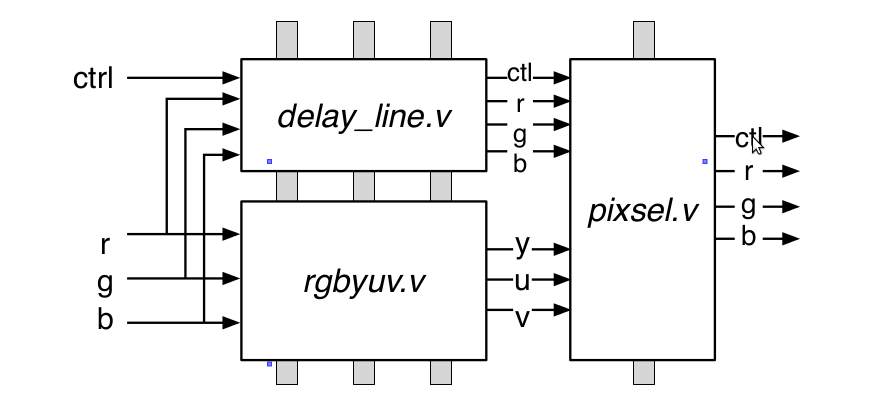
\includegraphics[width=\textwidth]{overall.png}
\caption{Design Diagram}
\label{fig:overall}
\end{figure}
There are 3 modules in this design. They are \textbf{\emph{delay\underline{ }line}}, \textbf{\emph{rgbyuv}} and \textbf{\emph{pixsel}}. Basically, \textbf{\emph{rgbyuv}} is used to convert RGB signals from a camera to YUV; \textbf{\emph{Delay\underline{ }line}} module is used to align signal in order to synchronize related input and control signal; Module \textbf{\emph{pixsel}} is used to select wanted signal from the previous two module according to control signal, output it to the top module, and then display on the screen.

%=====================================================================
\subsection{Structure of the rest of the paper}
The rest of the paper first describes the verilog implementations of \textbf{\emph{Task 1: rgbyuv Module}} in \emph{Section \ref{sec:task1}}, \textbf{\emph{Task 2: delay\underline{ }line Module}} in \emph{Section \ref{sec:task2}}; And \emph{Section \ref{sec:task34}} presents the experimental results \textbf{\emph{pixels}} module's selections and color effects. Lastly, \emph{Section \ref{sec:concl}} presents our conclusions and discussions.
%=====================================================================


\section{Task 1: rgbyuv Module}
\label{sec:task1}

%=====================================================================

\subsection{Verilog Code rgbyuv.v Non-pipelined}
\lstset {
    language=Verilog,
    backgroundcolor=\color{black!5},
    basicstyle=\ttfamily\footnotesize,
    numbers=left,
    numberstyle=\tiny,
    frame=single
}
{\linespread{0.75}
\begin{lstlisting}
ry<=((RY_COEF * red_r + GY_COEF * grn_r + BY_COEF * blu_r)>>>8)+16;
ru<=((RU_COEF * red_r + GU_COEF * grn_r + BU_COEF * blu_r)>>>8)+128;
rv<=((RV_COEF * red_r + GV_COEF * grn_r + BV_COEF * blu_r)>>>8)+128;
\end{lstlisting}
\par}
Synthesize this top module and check the synthesis report. Under the synthesis report, there is a device utilization summary. It shows that, 9 DSP blocks are in utilization.
\begin{figure}[H]
\centering
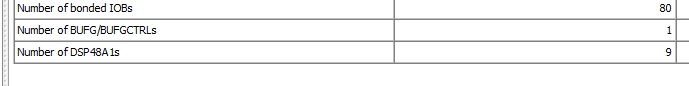
\includegraphics[width=\textwidth]{DSP9.jpg}
\caption{DSP Blocks}
\end{figure}
In the synthesis report, the maximum frequency is 77.873MHz.
\begin{figure}[H]
\centering
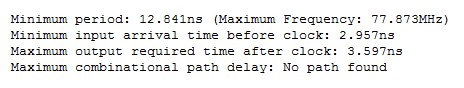
\includegraphics[width=0.7\textwidth]{77.jpg}
\caption{Frequency 77.873MHz}
\end{figure}

\subsection{Verilog Code rgbyuv.v with 2-stage pipelines}
If we simply add one more stage, which will result in a 2-stage pipelined computation steps. The pipeline diagram is shown below.
\begin{figure}[H]
\centering
\includegraphics[width=\textwidth]{2stage.jpg}
\caption{2-stage pipeline}
\label{fig:2stage}
\end{figure}


{\linespread{0.75}
\begin{lstlisting}
ry <= RY_COEF * red_r + GY_COEF * grn_r + BY_COEF * blu_r;
ru <= RU_COEF * red_r + GU_COEF * grn_r + BU_COEF * blu_r;
rv <= RV_COEF * red_r + GV_COEF * grn_r + BV_COEF * blu_r;
o_y <= (ry >>> 8) + 16;
o_u <= (ru >>> 8) + 128;
o_v <= (rv >>> 8) + 128;
\end{lstlisting}
\par}
After registers \emph{ry, ru, rv} inserted in the computation procedure, which split the step into a 2-stage pipelines like what is shown in Figure \ref{fig:2stage}. In the synthesis report, the maximum frequency is 96.034MHz.
\begin{figure}[H]
\centering
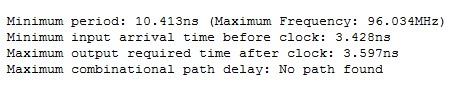
\includegraphics[width=0.7\textwidth]{96.jpg}
\caption{Frequency 96.034MHz}
\end{figure}
Compared to the previous two, the last implementation, which has 3 pipeline stages, is much better and manage to achieve 108MHz.
\subsection{Verilog Code rgbyuv.v with 3-stage pipelines}
\begin{figure}[H]
\centering
\includegraphics[width=\textwidth]{3stage.jpg}
\caption{3-stage pipeline}
\end{figure}
The multiplications part is the critical path for the whole pipelines among previous \textbf{\emph{rgbyuv.v}} implementations. So they are mostly likely to be splitted and it is supposed to give us a good result.
{\linespread{0.75}
\begin{lstlisting}
ry1 <= RY_COEF * red_r;
ry2 <= GY_COEF * grn_r;
ry3 <= BY_COEF * blu_r;
ru1 <= RU_COEF * red_r;
ru2 <= GU_COEF * grn_r;
ru3 <= BU_COEF * blu_r;
rv1 <= RV_COEF * red_r;
rv2 <= GV_COEF * grn_r;
rv3 <= BV_COEF * blu_r;
ry <= ry1 + ry2 + ry3;
ru <= ru1 + ru2 + ru3;
rv <= rv1 + rv2 + rv3;
o_y <= (ry >>> 8) + 16;
o_u <= (ru >>> 8) + 128;
o_v <= (rv >>> 8) + 128;
\end{lstlisting}
\par}
The critical path was splitted into 3 similar part, which results in a high frequency achievement.\\
This time, the frequency is 209.249MHz.
\begin{figure}[H]
\centering
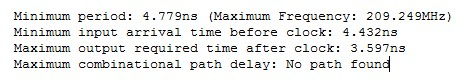
\includegraphics[width=0.7\textwidth]{209.jpg}
\caption{Frequency 209.249MHz}
\end{figure}
One last improvement, if we put all of the operations into pipelines, the maximum frequency will reach about 456MHz. However, too many pipeline stages will cause more complicated signal alignment in next section, which is \emph{section \ref{sec:task2}}.
\begin{figure}[H]
\centering
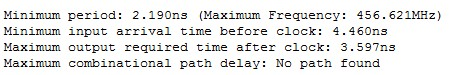
\includegraphics[width=0.7\textwidth]{456.jpg}
\caption{Frequency 456.621MHz}
\end{figure}

\subsection{skin pixel detection with a 4-stage pipeline}
{\linespread{0.75}
\begin{lstlisting}
      //add one more stage
      p_y <= (ry >>> 8) + 16;
      p_u <= (ru >>> 8) + 128;
      p_v <= (rv >>> 8) + 128;
      o_y <= p_y; o_u <= p_u; o_v <= p_v;
    end
  end // always @ (posedge clk)
  
  always @(posedge clk) begin
    if (rst) begin
      skind <= 1'b0;
    end else begin
      if (73 <= p_u && p_u <= 122 && 132 <= p_v && p_v <= 173) begin
        skind <= 1'b1;
      end else begin
        skind <= 1'b0;
      end
    end
  end // always @ (posedge clk)
\end{lstlisting}
\par}
If a pixel is detected having a skin-like color by using YUV analysis, a 1-bit register \emph{skind} will be asserted to 1, otherwise 0.
%====================================

\section{Task 2: delay\underline{ }line Module}
\label{sec:task2}
\subsection{Verilog Code delay\underline{ }line.v}
%\begin{multicols}{2}
{\linespread{0.75}
\begin{lstlisting}[numbers=left,multicols=2]
always @(posedge clk) begin
    if(rst) begin
      in_r_p1 <=8'd0;
      in_r_p2 <= 8'd0;
      in_r_p3 <= 8'd0;
      in_r_p4 <= 8'd0;
      out_r <= 8'd0;
      
      in_g_p1 <=8'd0;
      in_g_p2 <= 8'd0;
      in_g_p3 <= 8'd0;
      in_g_p4 <= 8'd0;
      out_g <= 8'd0;
      
      in_b_p1 <=8'd0;
      in_b_p2 <= 8'd0;
      in_b_p3 <= 8'd0;
      in_b_p4 <= 8'd0;
      out_b <= 8'd0;
      
      in_c_p1 <=8'd0;
      in_c_p2 <= 8'd0;
      in_c_p3 <= 8'd0;
      in_c_p4 <= 8'd0;
      out_c <= 8'd0;
    end else begin
      in_r_p1 <= in_r;
      in_r_p2 <= in_r_p1;
      in_r_p3 <= in_r_p2;
      in_r_p4 <= in_r_p3;
      out_r   <= in_r_p3;
		  
      in_g_p1 <= in_g;
      in_g_p2 <= in_g_p1;
      in_g_p3 <= in_g_p2;
      in_g_p4 <= in_g_p3;
      out_g   <= in_g_p4;
      
      in_b_p1 <= in_b;
      in_b_p2 <= in_b_p1;
      in_b_p3 <= in_b_p2;
      in_b_p4 <= in_b_p3;
      out_b   <= in_b_p4;
      
      in_c_p1 <= in_c;
      in_c_p2 <= in_c_p1;
      in_c_p3 <= in_c_p2;
      in_c_p4 <= in_c_p3;
      out_c   <= in_c_p4;
    end // else: !if(rst)
  end // always @ (posedge clk)
endmodule // delay_line
\end{lstlisting}
\par}
As we can see from the module name, \textbf{\emph{delay\underline{}line}} is used to delay the input signal by using pipelines. Because we are currently using a 5-stage pipelined \textbf{\emph{rgbyuv.v}}, \textbf{\emph{delay\underline{}line}} are supposed to have the same pipelining stages as it.

\section{Task 3 \& 4: Logically Display}
\label{sec:task34}
%=====================================================================
Task 3 and task 4 are combined together, because task 4 is roughly improvement of task 3 with more pixel operations.
\subsection{Verilog Code pixsel.v}
\lstset {
    language=Verilog,
    backgroundcolor=\color{black!5},
    basicstyle=\ttfamily\footnotesize,
    numbers=left,
    numberstyle=\tiny,
    frame=single
}
{\linespread{0.75}
\begin{lstlisting}
  always @(posedge clk) begin
    if(rst) begin
      out_r <= 8'd0;
      out_g <= 8'd0;
      out_b <= 8'd0;
      out_ctrl <= 3'd0;
      end else begin
        case(in_swt)
          1 : begin
            out_r <= in_y; out_g <= in_y; out_b <= in_y;
          end
          2 : begin
            out_r <= in_u; out_g <= in_u; out_b <= in_u;
          end
          4 : begin
            out_r <= in_v; out_g <= in_v; out_b <= in_v;
          end
          /*8 : begin
            if (in_skin) begin
              out_r <= in_y; out_g <= in_y; out_b <= in_y;
            end else begin
              out_r <= 1'b0; out_g <= 1'b0; out_b <= 1'b0;
            end
          end*/
          //display with maximum green
          8 : begin
            if (in_skin) begin
              out_r <= min_r; out_g <= max_g; out_b <= min_b;
            end else begin
              out_r <= in_r; out_g <= in_g; out_b <= in_b;
            end
          end
          //display with maximum red
          16 : begin
            if (in_skin) begin
              out_r <= max_r; out_g <= min_g; out_b <= min_b;
            end else begin
              out_r <= in_r; out_g <= in_g; out_b <= in_b;
            end
          end
          //display with maximum blue
          32 : begin
            if (in_skin) begin
              out_r <= min_r; out_g <= min_g; out_b <= max_b;
            end else begin
              out_r <= in_r; out_g <= in_g; out_b <= in_b;
            end
          end
          //display with maximum red, green and blue
          64 : begin
            if (in_skin) begin
              out_r <= max_r; out_g <= max_g; out_b <= max_b;
            end else begin
              out_r <= in_r; out_g <= in_g; out_b <= in_b;
            end
          end
          //display original skin color. otherwise max r & g & b
          128 : begin
            if (in_skin) begin
              out_r <= in_r; out_g <= in_g; out_b <= in_b;
            end else begin
              out_r <= max_r; out_g <= max_g; out_b <= max_b;
            end
          end
          //for fun
          255 : begin
            if (in_skin) begin
              out_r <= in_r; out_g <= in_g; out_b <= in_b;
            end else begin
              out_r <= min_r; out_g <= min_g; out_b <= min_b;
            end
          end
          default : begin
            out_r <= in_r; out_g <= in_g; out_b <= in_b;
          end
        endcase // case (in_swt)
        out_ctrl <= in_c;
      end // else: !if(rst)
  end // always @ (posedge clk)
\end{lstlisting}
\par}
A one-hot strategy was employed to control the pixel selections. More details are given below.
\textbf{\emph{Case 1, 2, 4:}}\\
The screen turned black and white in case 1, because there is no color output from \emph{pixsel.v}, except \emph{y}, which is the luminance or brightness of a pixel; The screen turned inverted darkness and grey in switch 2 and turning palely grey in switch 4.\\
\textbf{\emph{Case 8, 16, 32:}}\\
In task 3, fpga is supposed to show those pixels detected as skin ones. The others will be blocked, which results that only skin parts will be shown on the screen.\\
But the result will not be very good: there will be many incorrect outputs, such like fluorescent lamp, white wall, since we are currently using a basic skin color detection algorithm.
In task 4, instead of blocking other pixels and displaying skin ones, fpga is supposed to change skin colors by replace original pixels' data with different colors and keep the other pixels unchanged.
{\linespread{0.75}
\begin{lstlisting}
  wire [8:0]         max_r = ((in_r + 64)<255) ? in_r + 64 : 255;
  wire [8:0]         min_r = ((in_r - 32)>0)   ? in_r - 32 : 0;
  wire [8:0]         max_g = ((in_g + 64)<255) ? in_g + 64 : 255;
  wire [8:0]         min_g = ((in_g - 32)>0)   ? in_g - 32 : 0;
  wire [8:0]         max_b = ((in_b + 64)<255) ? in_b + 64 : 255;
  wire [8:0]         min_b = ((in_b - 32)>0)   ? in_b - 32 : 0;
\end{lstlisting}
\par}
{\linespread{0.75}
\begin{lstlisting}
out_r <= min_r; out_g <= max_g; out_b <= min_b;
\end{lstlisting}
\par}
If max\underline{ }g was used to replace out\underline{ }g, the skin pixels will be replaced by green pixels.
{\linespread{0.75}
\begin{lstlisting}
out_r <= max_r; out_g <= min_g; out_b <= min_b;
\end{lstlisting}
\par}
If max\underline{ }r was used to replace out\underline{ }r, the skin pixels will be replaced by red pixels.
{\linespread{0.75}
\begin{lstlisting}
out_r <= min_r; out_g <= min_g; out_b <= max_b;
\end{lstlisting}
\par}
If max\underline{ }b was used to replace out\underline{ }b, the skin pixels will be replaced by blue pixels.

\textbf{\emph{Case 64, 128:}}\\
{\linespread{0.75}
\begin{lstlisting}
if (in_skin)
  out_r <= max_r; out_g <= max_g; out_b <= max_b;
else
  out_r <= in_r; out_g <= in_g; out_b <= in_b;
\end{lstlisting}
\par}
If all out\underline{ } were replaced by max\underline{ }, the skin pixels will become pale instead of original flesh or pink color.
{\linespread{0.75}
\begin{lstlisting}
if (in_skin)
  out_r <= in_r; out_g <= in_g; out_b <= in_b;
else
  out_r <= max_r; out_g <= max_g; out_b <= max_b;
\end{lstlisting}
\par}
Doing fun, after exchange these two line unblocking assignment, the skin pixels went out directly, and other pixels become greyer than before. But there is a side effect: some pixels on skin may not be detected as a skin pixel, which results that the whole skin looks darker than before. 

\textbf{\emph{Case 255:}}\\
{\linespread{0.75}
\begin{lstlisting}
if (in_skin)
  out_r <= in_r; out_g <= in_g; out_b <= in_b;
else
  out_r <= min_r; out_g <= min_g; out_b <= min_b;
\end{lstlisting}
\par}
This time, all the black color shined, and skin pixels were kept unchanged. It because we set, if a pixel is not a skin pixel, then it will be replaced by min\underline{ }r, min\underline{ }g and min\underline{ }b.
 
%=================================================================
\section{Conclusions and Future Work}
\label{sec:concl}
In this lab session, pipelining and signal aligning techniques were employed to process input signals from a camera. In addition, pixels selection and logical color conversion were applied to produce several special visual effects.

%=====================================================================
\subsection{\emph{Problems} occurred in our approach}
%\begin{figure}[H]
%\centering
%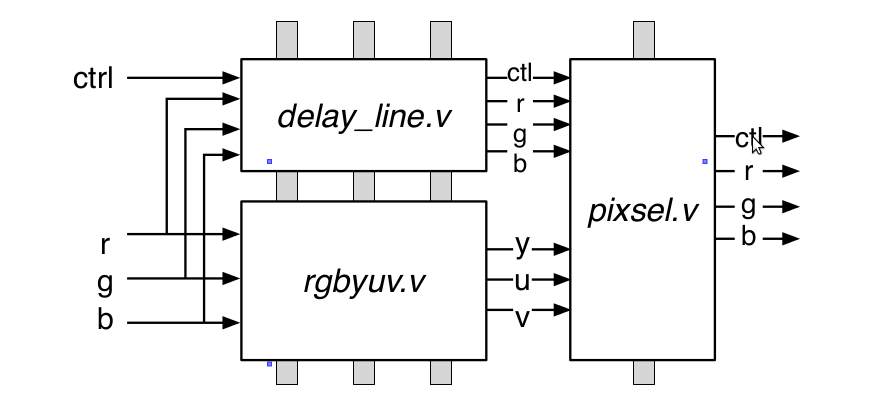
\includegraphics[width=\textwidth]{overall.png}
%\caption{Design Diagram}
%\end{figure}
From the Figure \ref{fig:overall} above, we can see that the output signals (ctl, r, g, b) of \textbf{\emph{delay\underline{ }line}} module need to be synchronous with the output signals (y, u, v) of \textbf{\emph{rgbyuv}} module. Sine a 4-stage pipeline was employed in \textbf{\emph{rgbyuv}} module, the \textbf{\emph{delay\underline{ }line}} module is also required to have a 4-stage pipeline.\\
If the number of stages in \textbf{\emph{delay\underline{ }line}} module is different from \textbf{\emph{rgbyuv}}, fpge would not generate video output to screen.\\
Because all the multiplications at the first stage in \textbf{\emph{rgbyuv.v}} will be the critical path for the whole pipelines. So if the most slow part in a pipeline is separated like the code above, it will result in a significant improvement on maximum frequency.\\
\subsection{Available \emph{Improvement}}
10 kinds of color effects were conducted based on skin color detection and YUV colorspace. Actually, more achievements are available. For example, one way is that we can change the skin color detect block to other color detect, and even more than color detection.\\
 Another way is that instead of using one-hot strategy, which will only have 8 features, we can actually add more features by changing the output with different color combinations like what was done in this report.\\
A pipelined \textbf{\emph{rgbyuv.v}} at a frequency of 456MHz was conducted during taks 1. But it was not employed during the synthesis procedure, because a pipeline with too many stages is redundant for this lab implementation.\\
\newpage
%=====================================================================

\section{Appendix}
\emph{Please ignore the time stamp on the right corner of each picture. There was something wrong with my camera.} 
\begin{multicols}{2}
\begin{figure}[H]
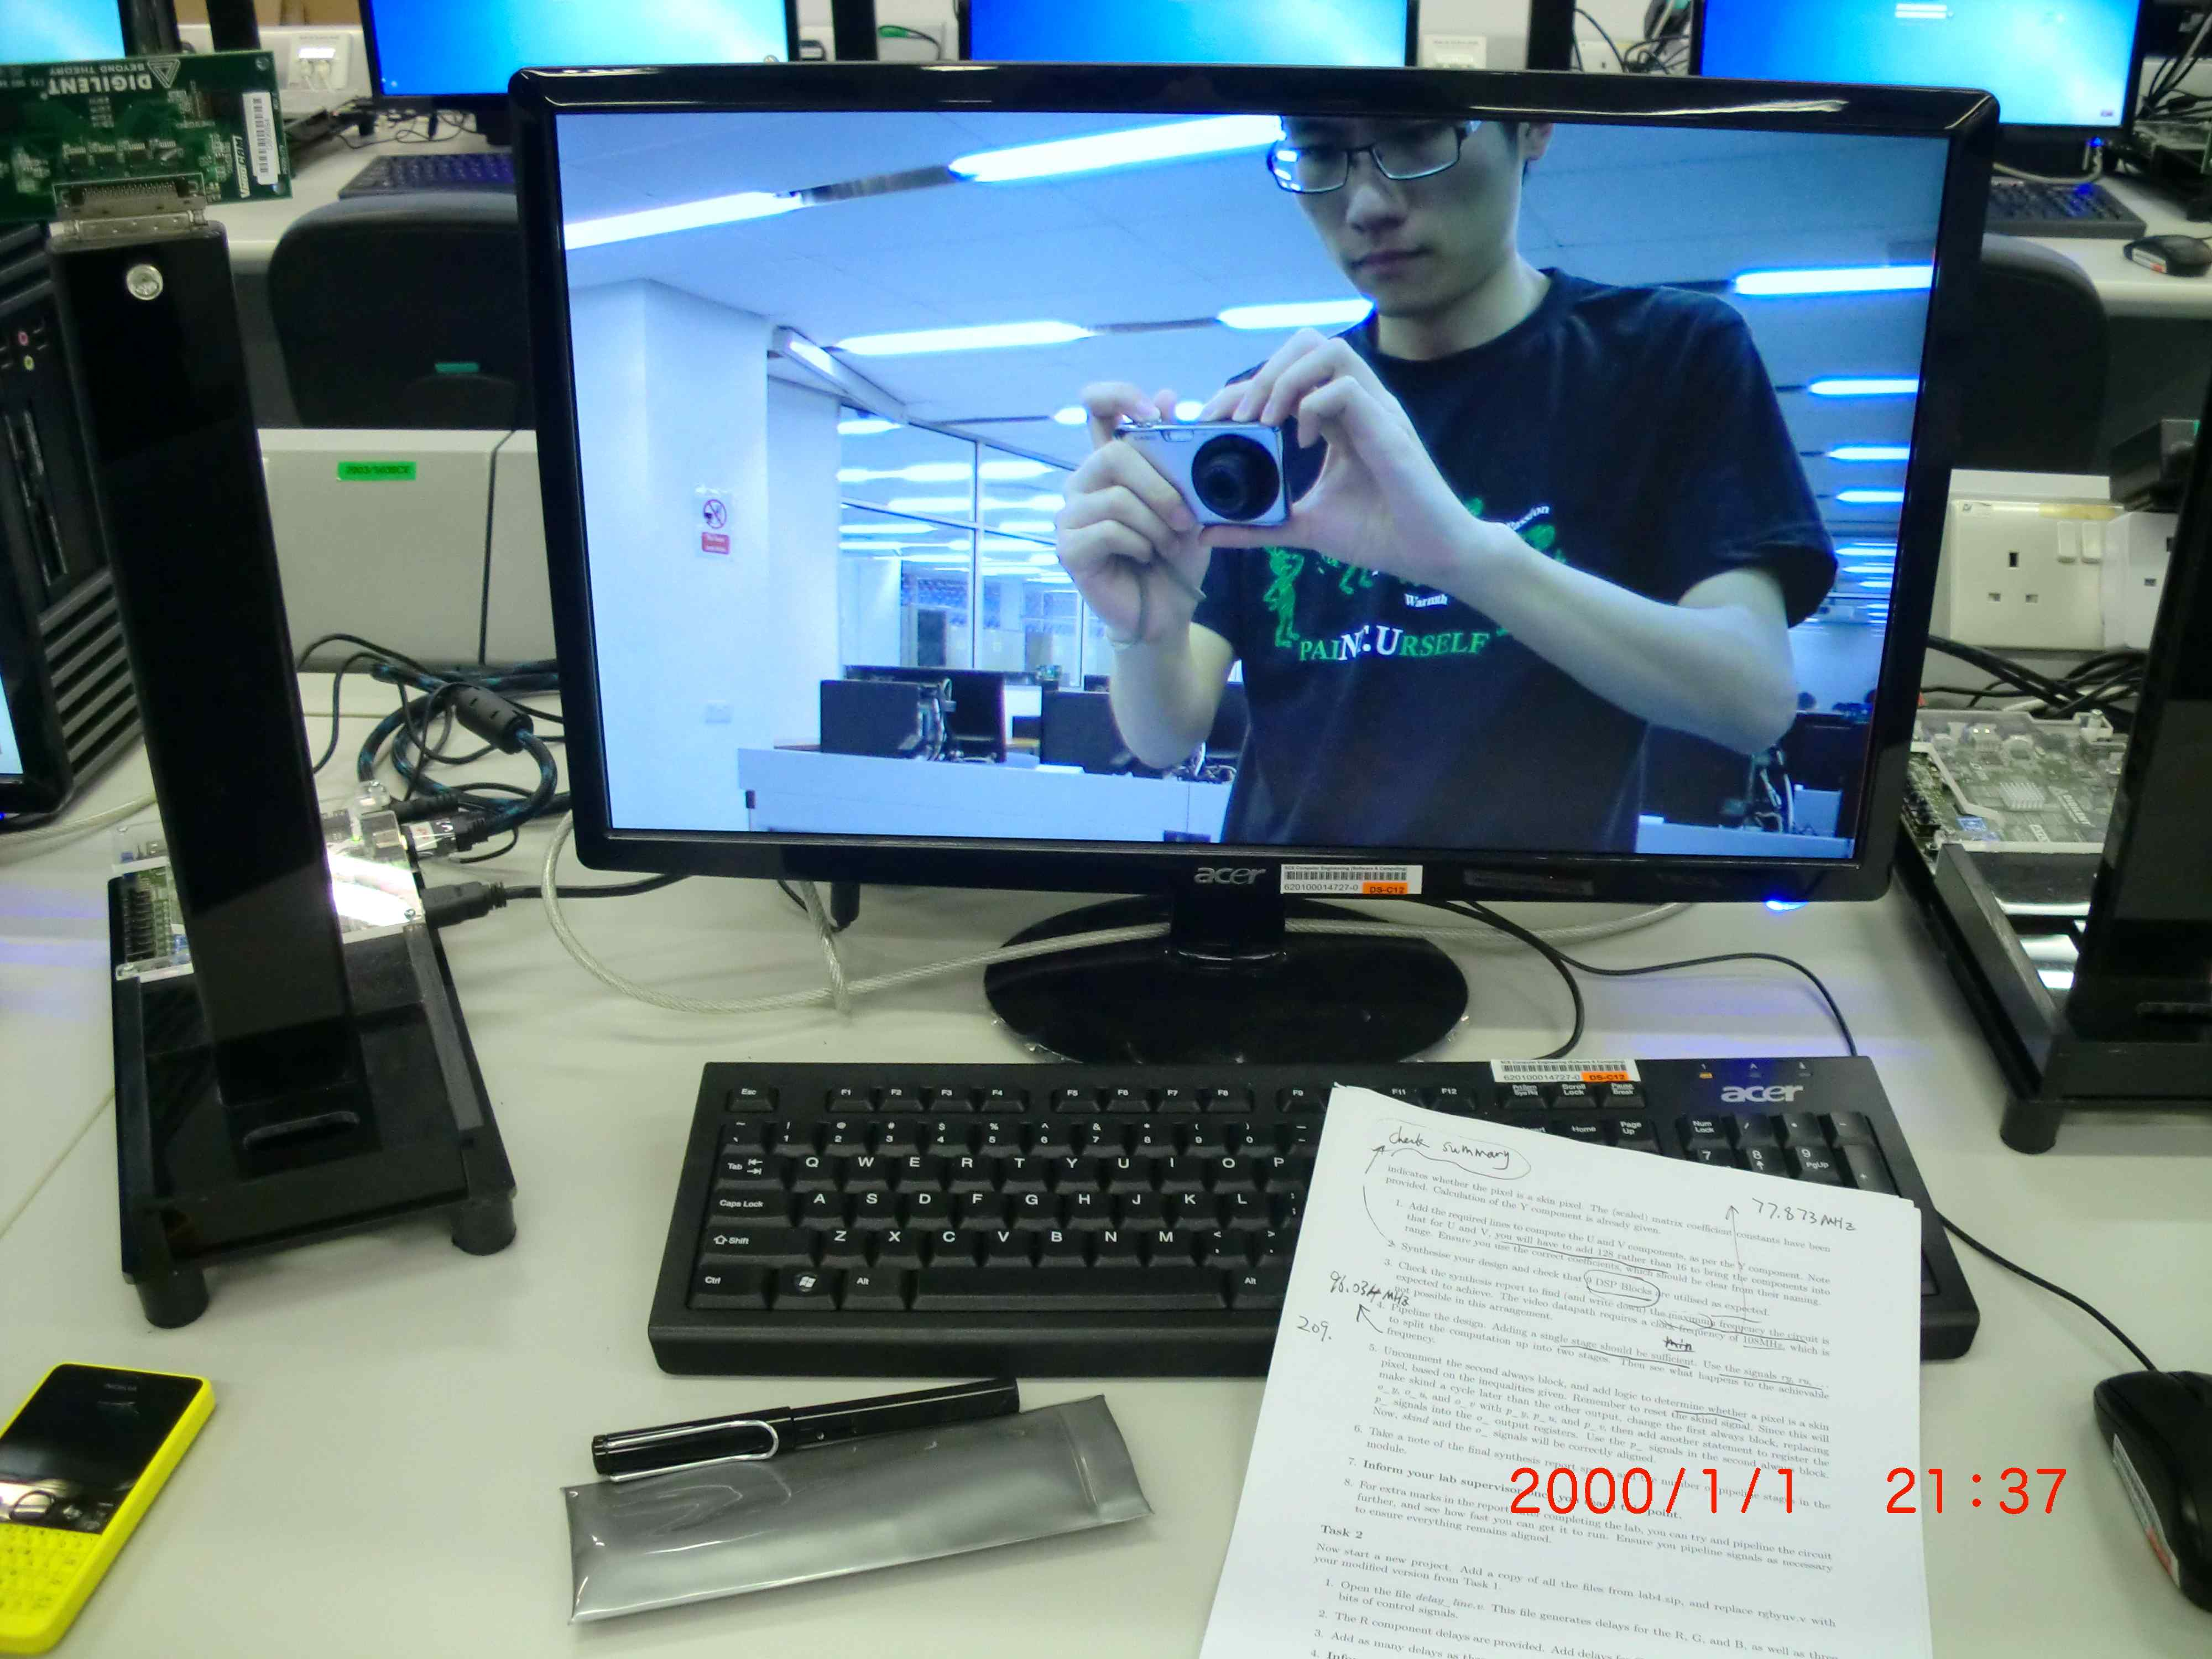
\includegraphics[width=0.5\textwidth]{a0.JPG}
\captionof{figure}{Case default}
\end{figure}
\begin{figure}[H]
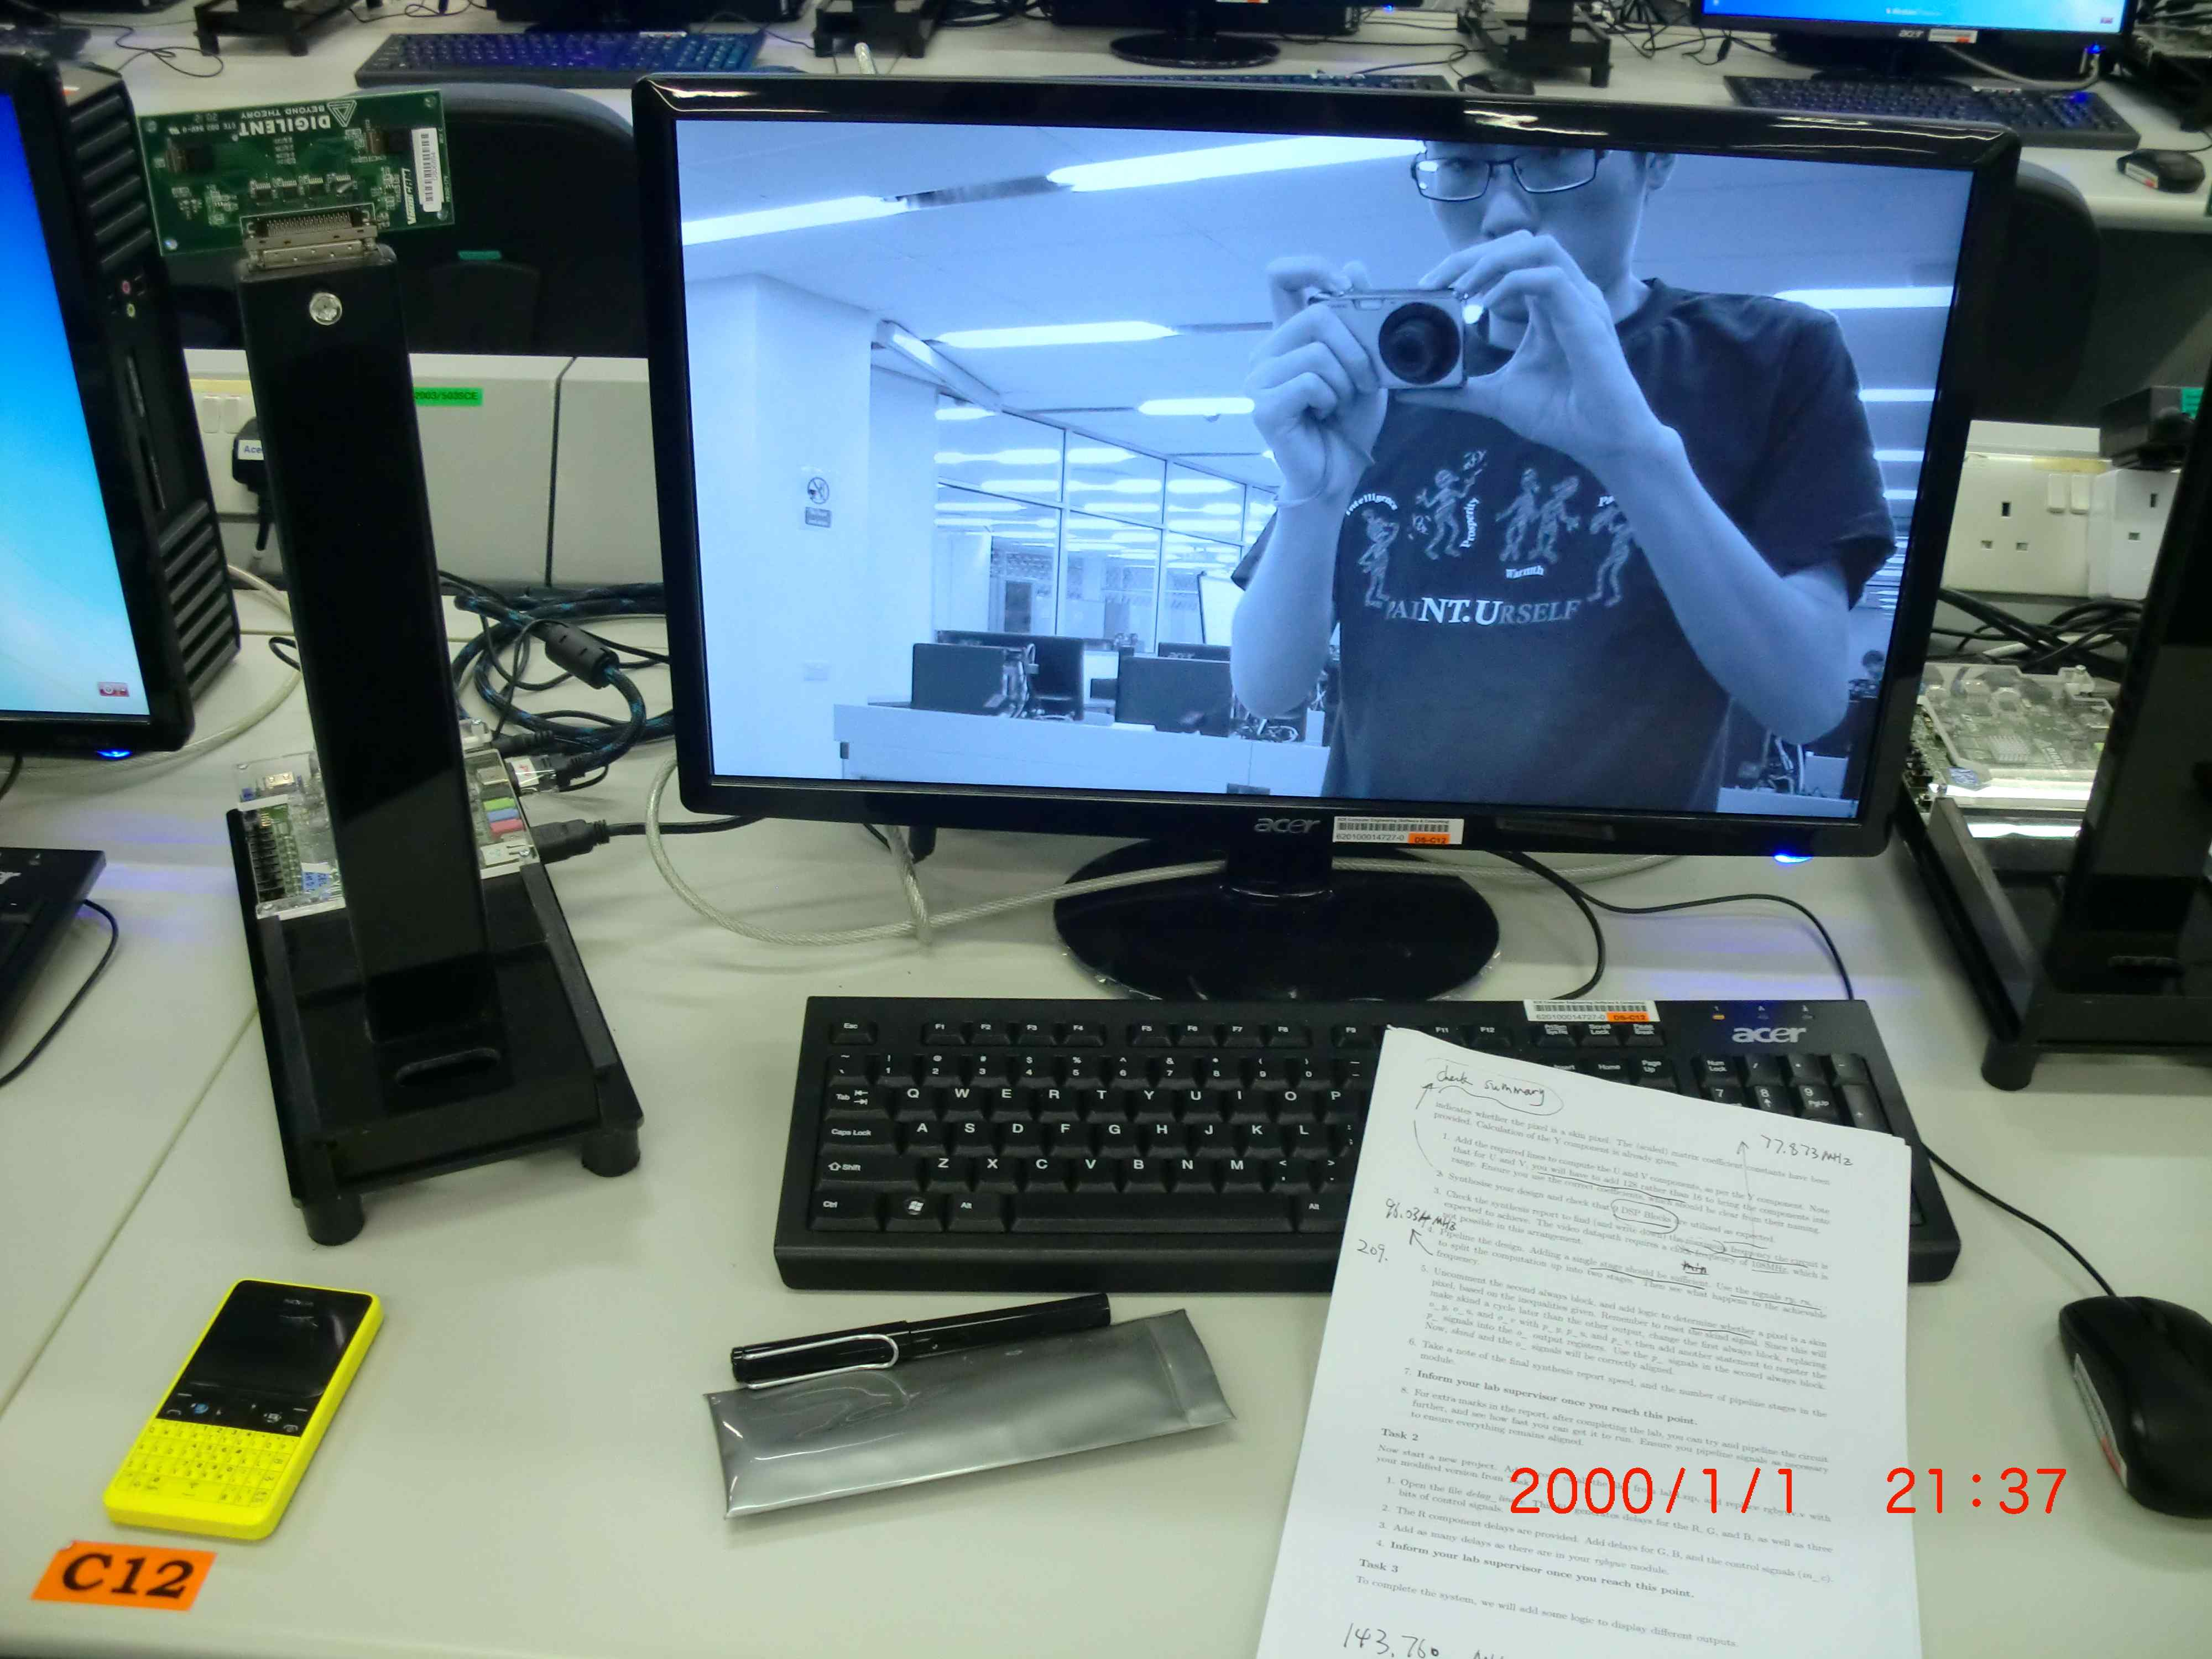
\includegraphics[width=0.5\textwidth]{a1.JPG}
\captionof{figure}{Case 1}
\end{figure}
\begin{figure}[H]
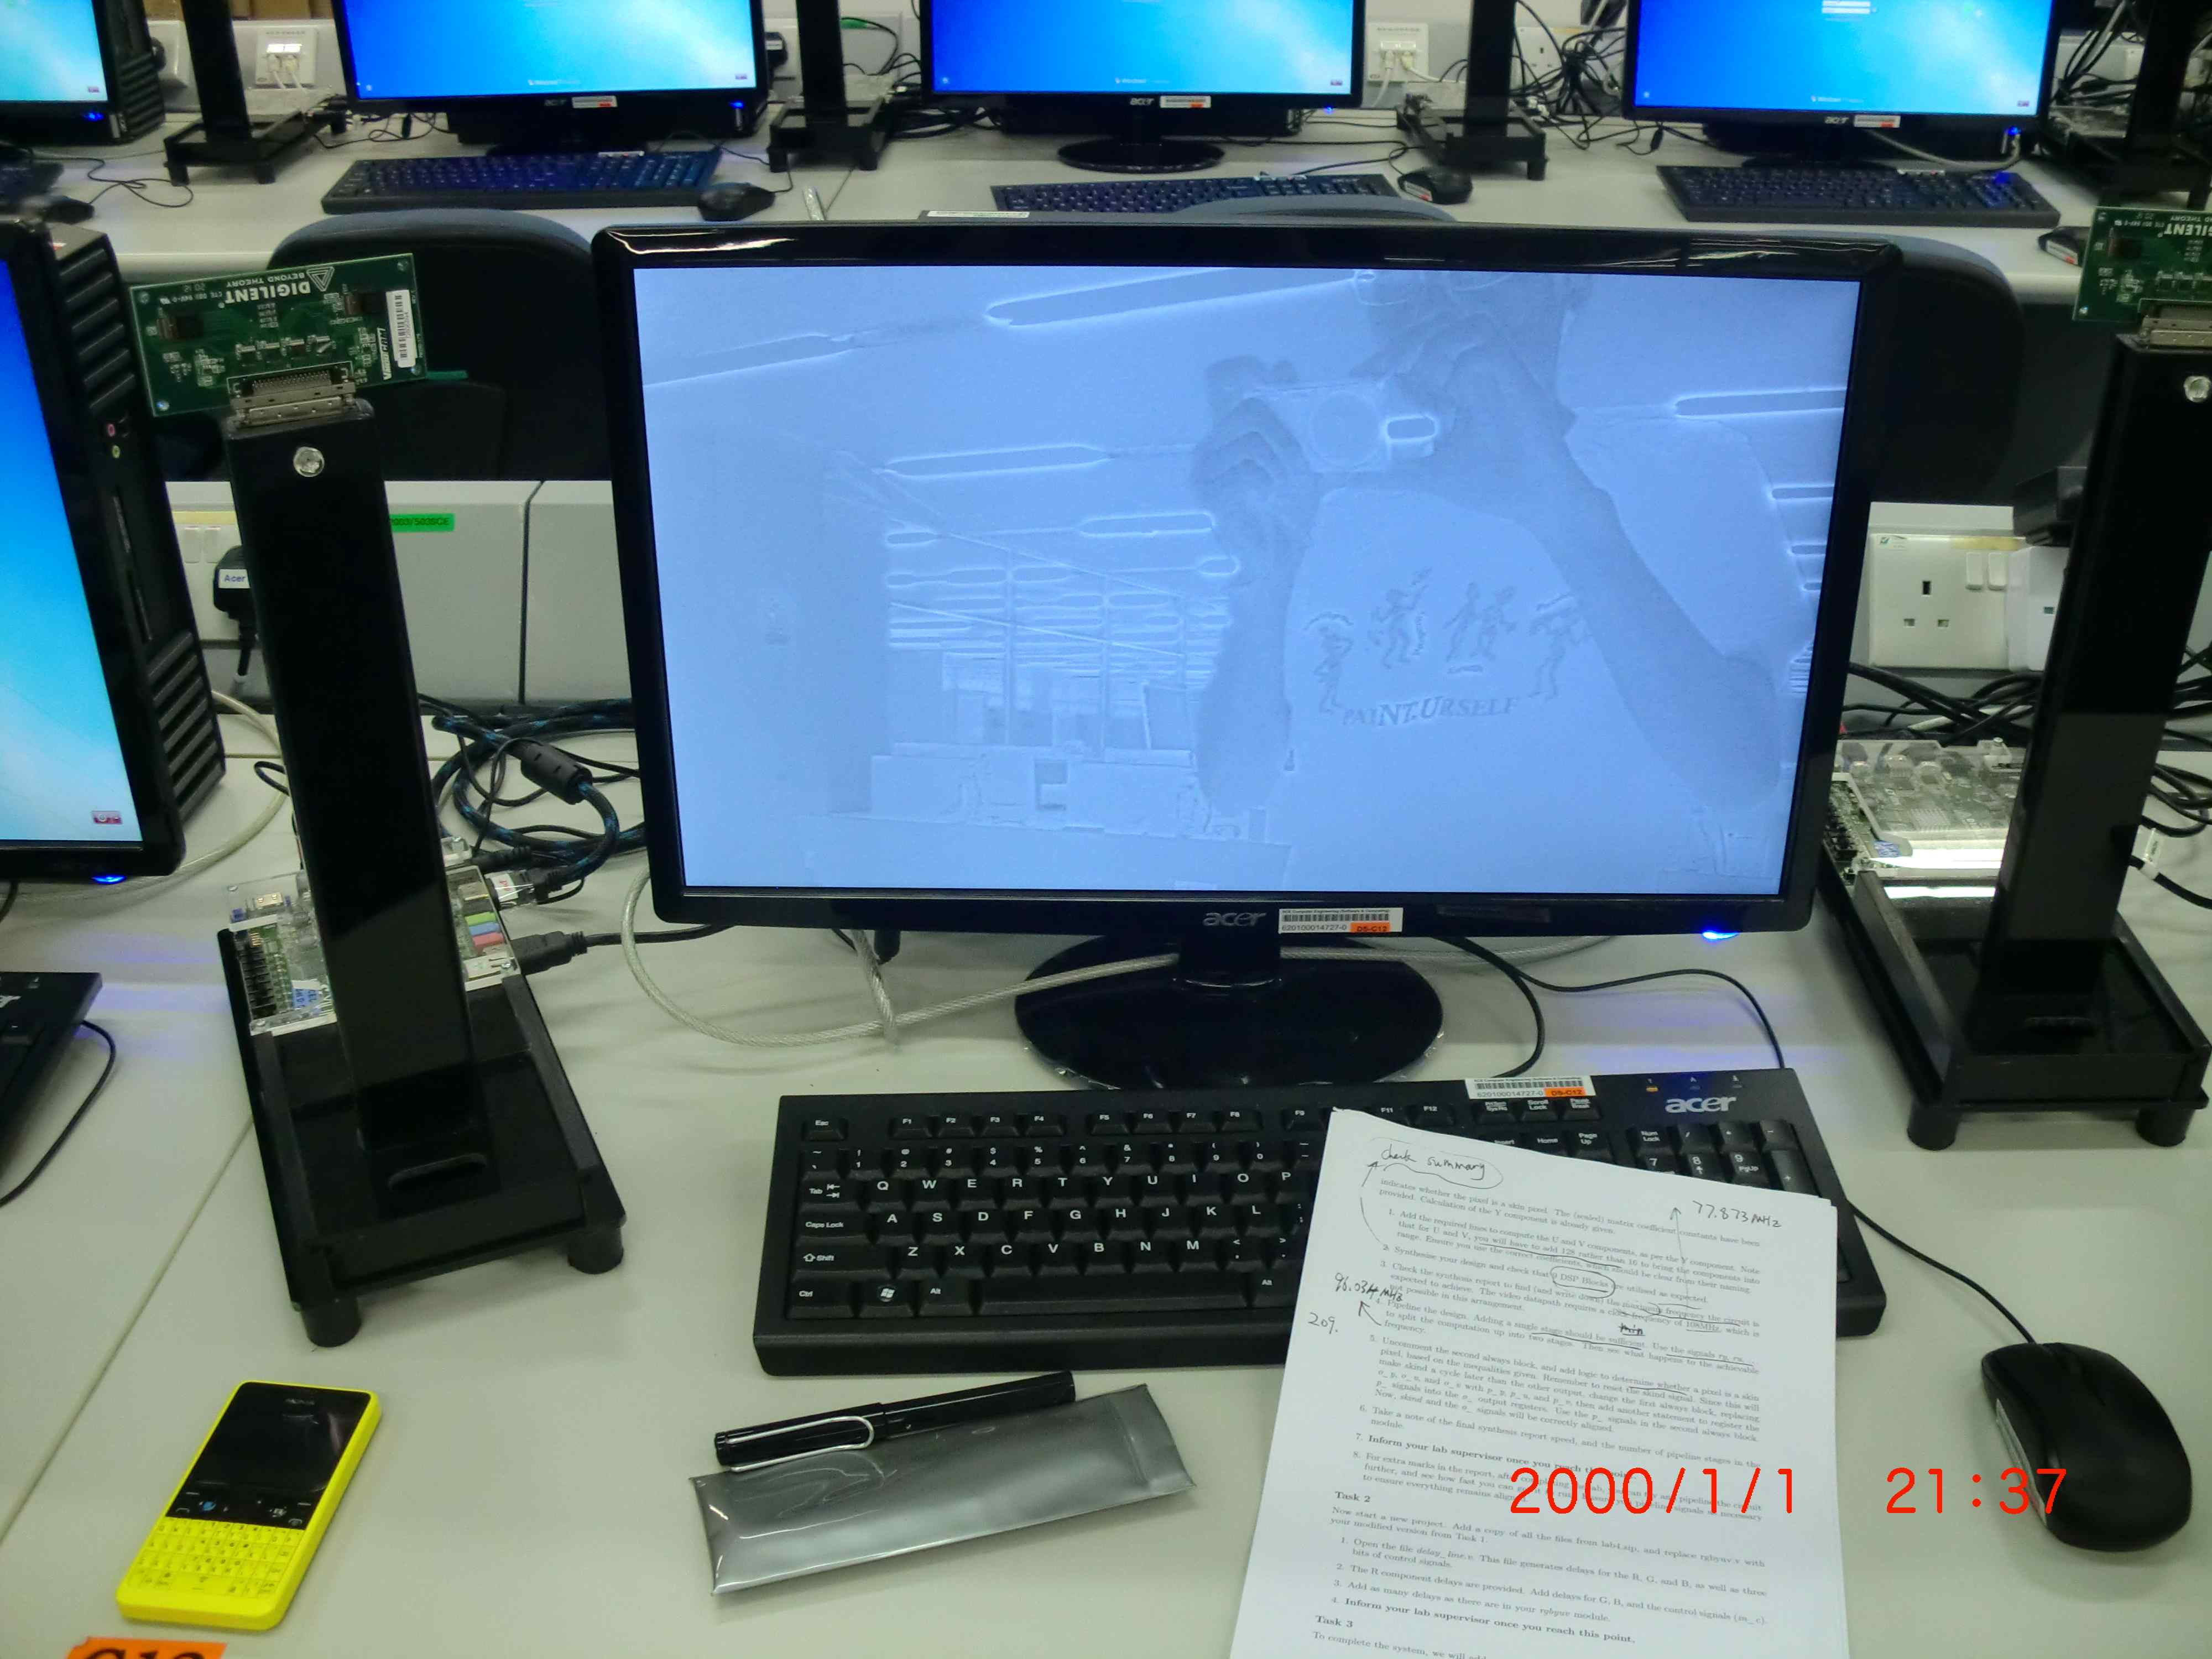
\includegraphics[width=0.5\textwidth]{a2.JPG}
\captionof{figure}{Case 2}
\end{figure}
\begin{figure}[H]
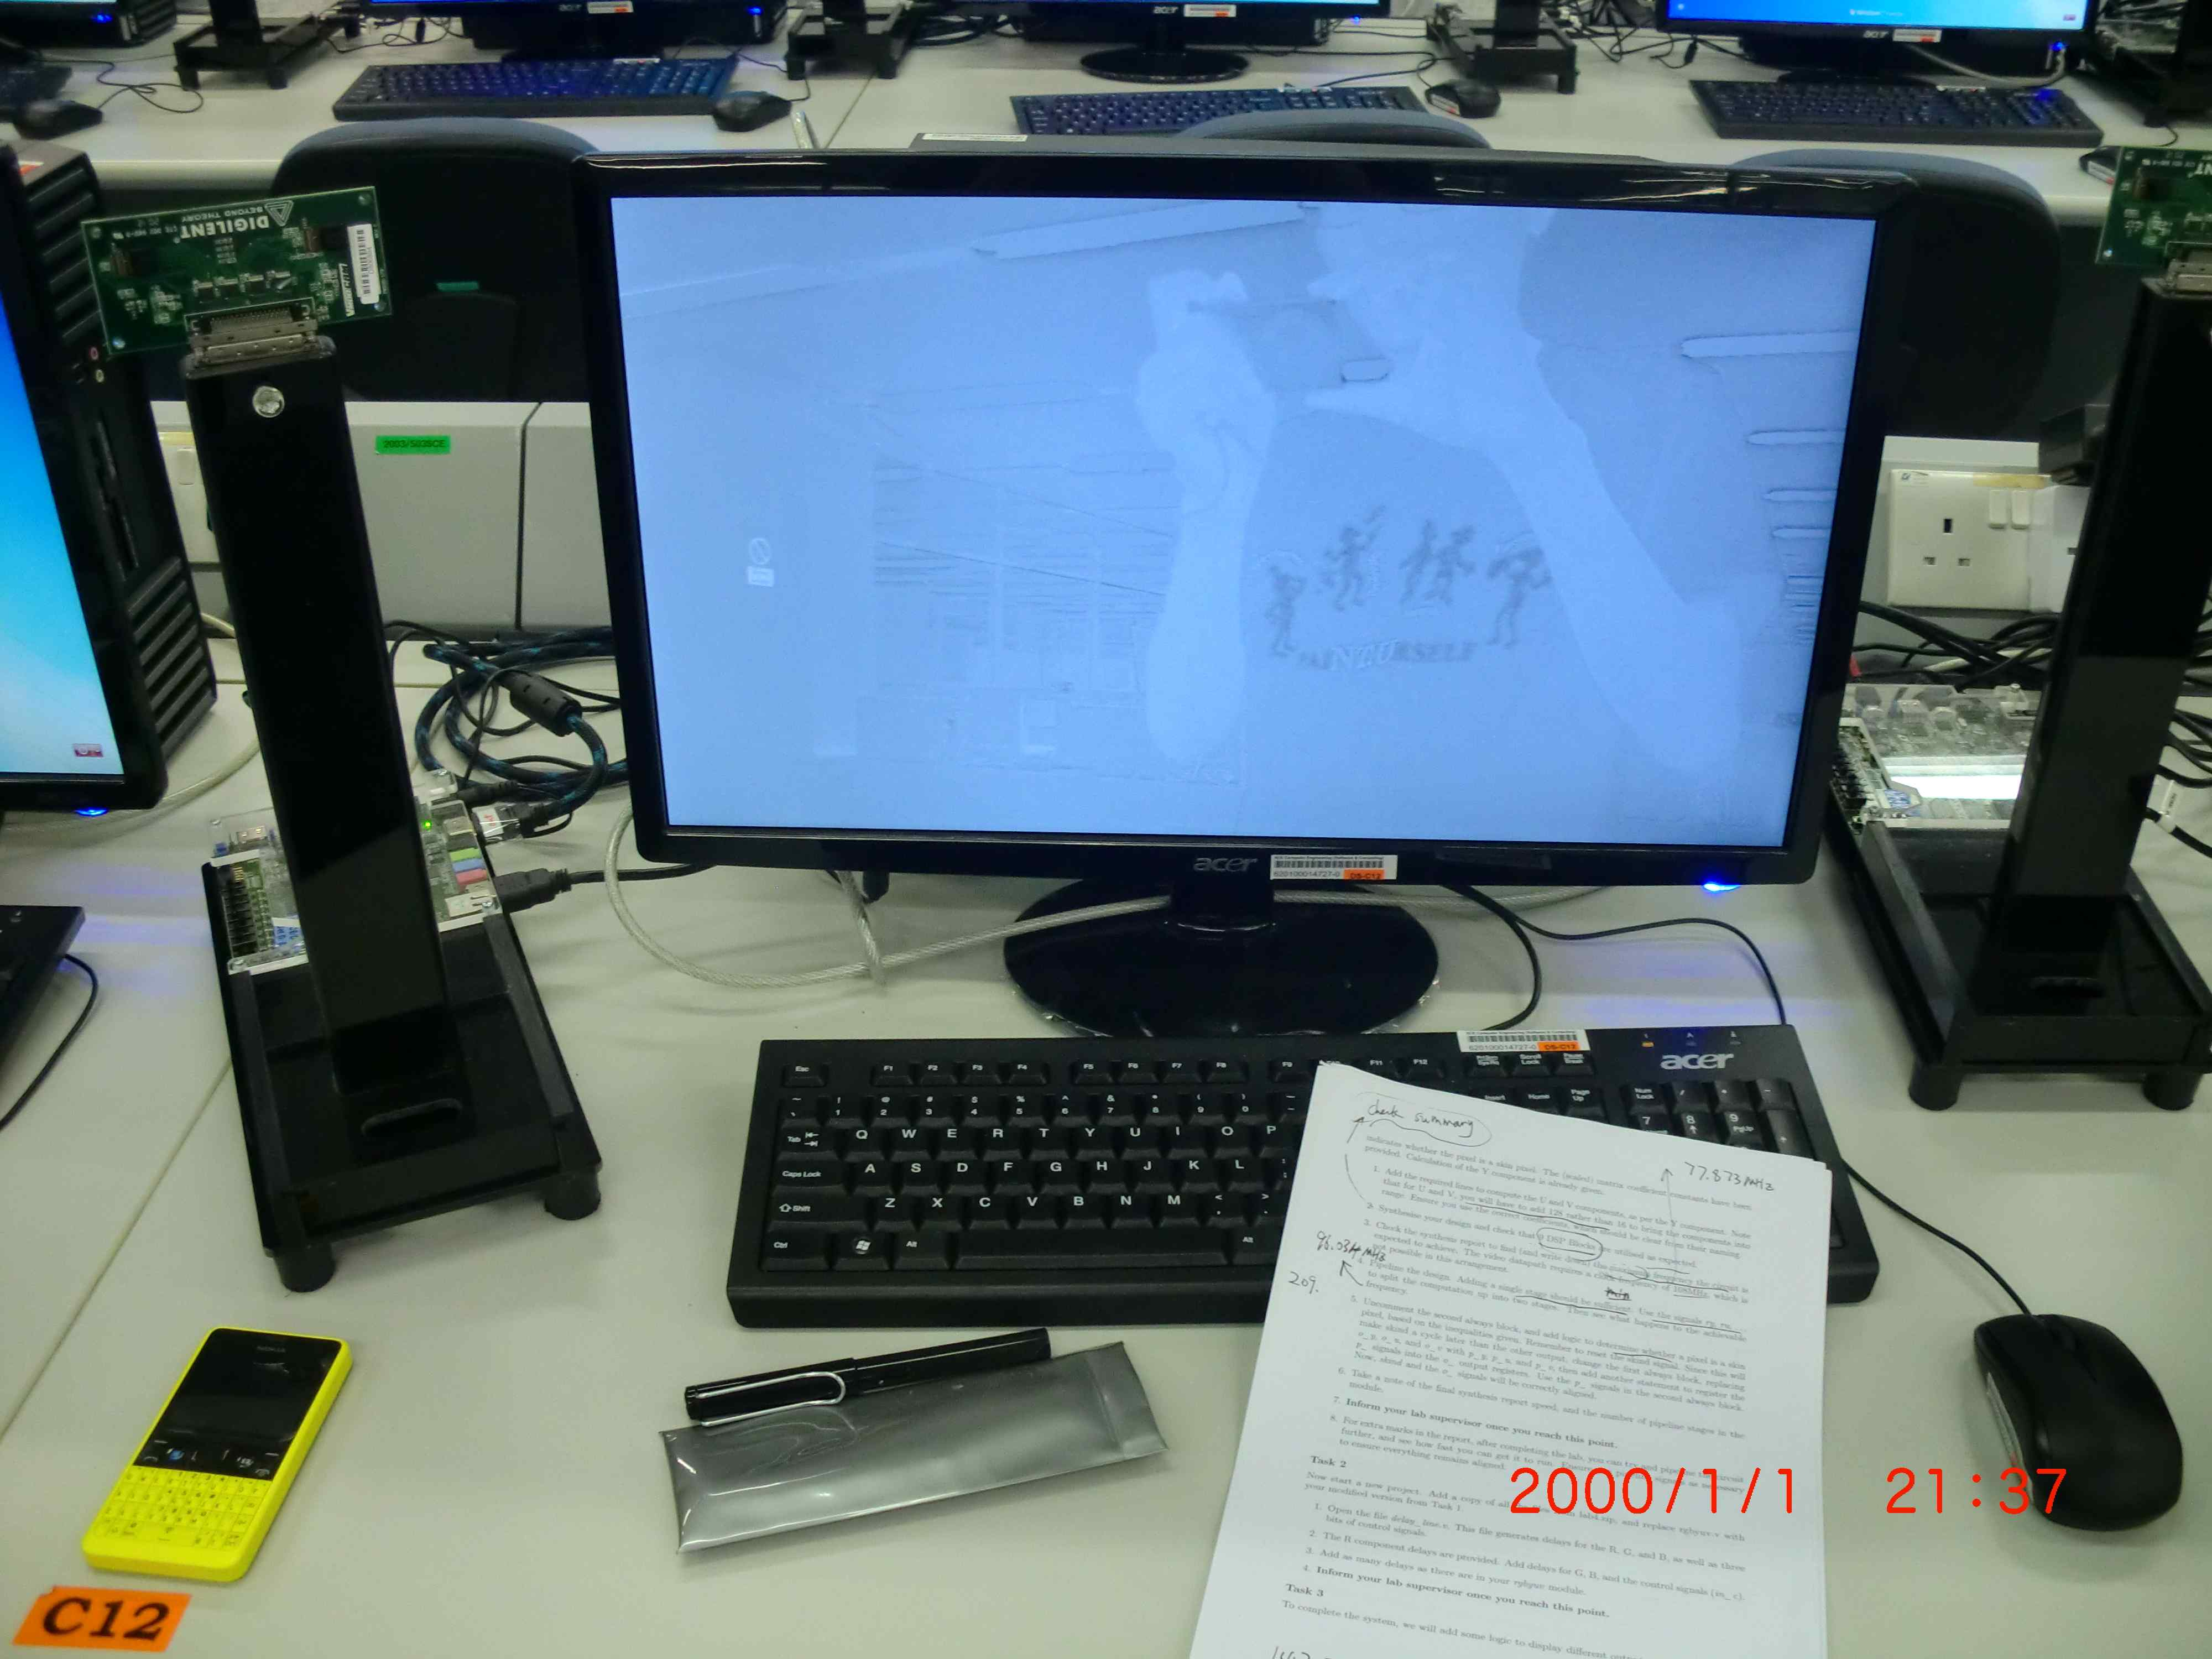
\includegraphics[width=0.5\textwidth]{a3.JPG}
\captionof{figure}{Case 4}
\end{figure}
\begin{figure}[H]
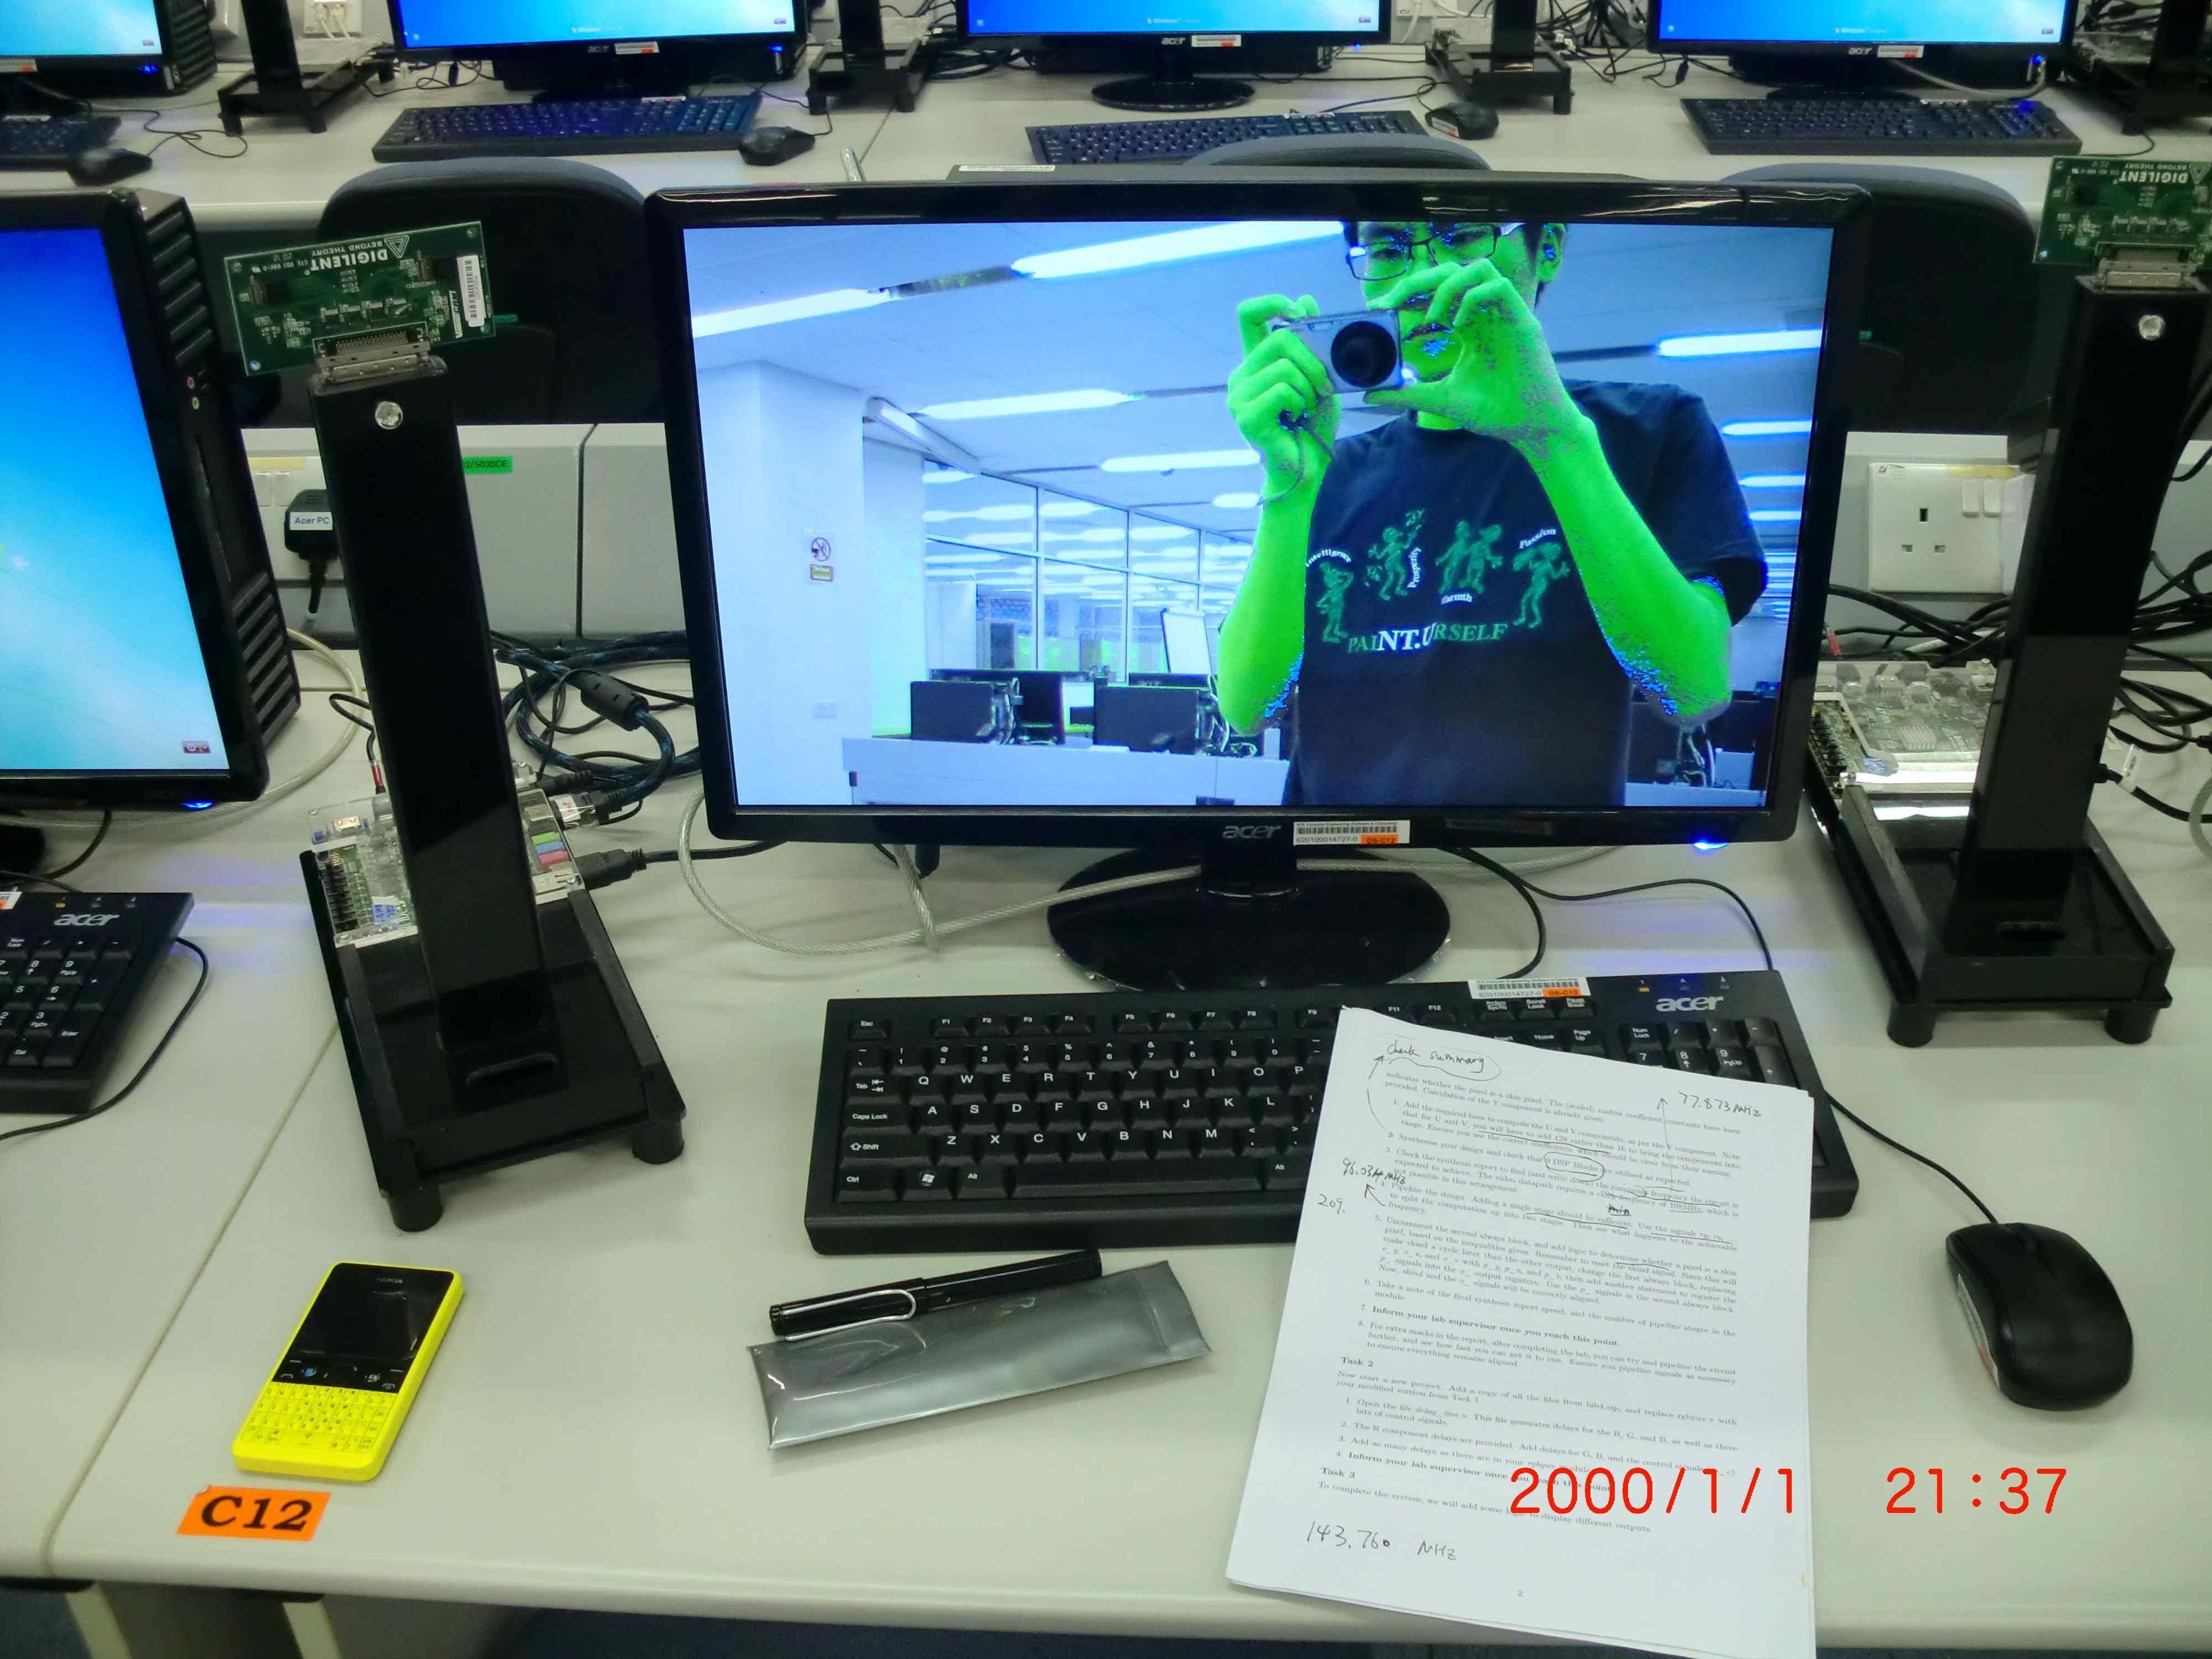
\includegraphics[width=0.5\textwidth]{a4.JPG}
\captionof{figure}{Case 8}
\end{figure}
\begin{figure}[H]
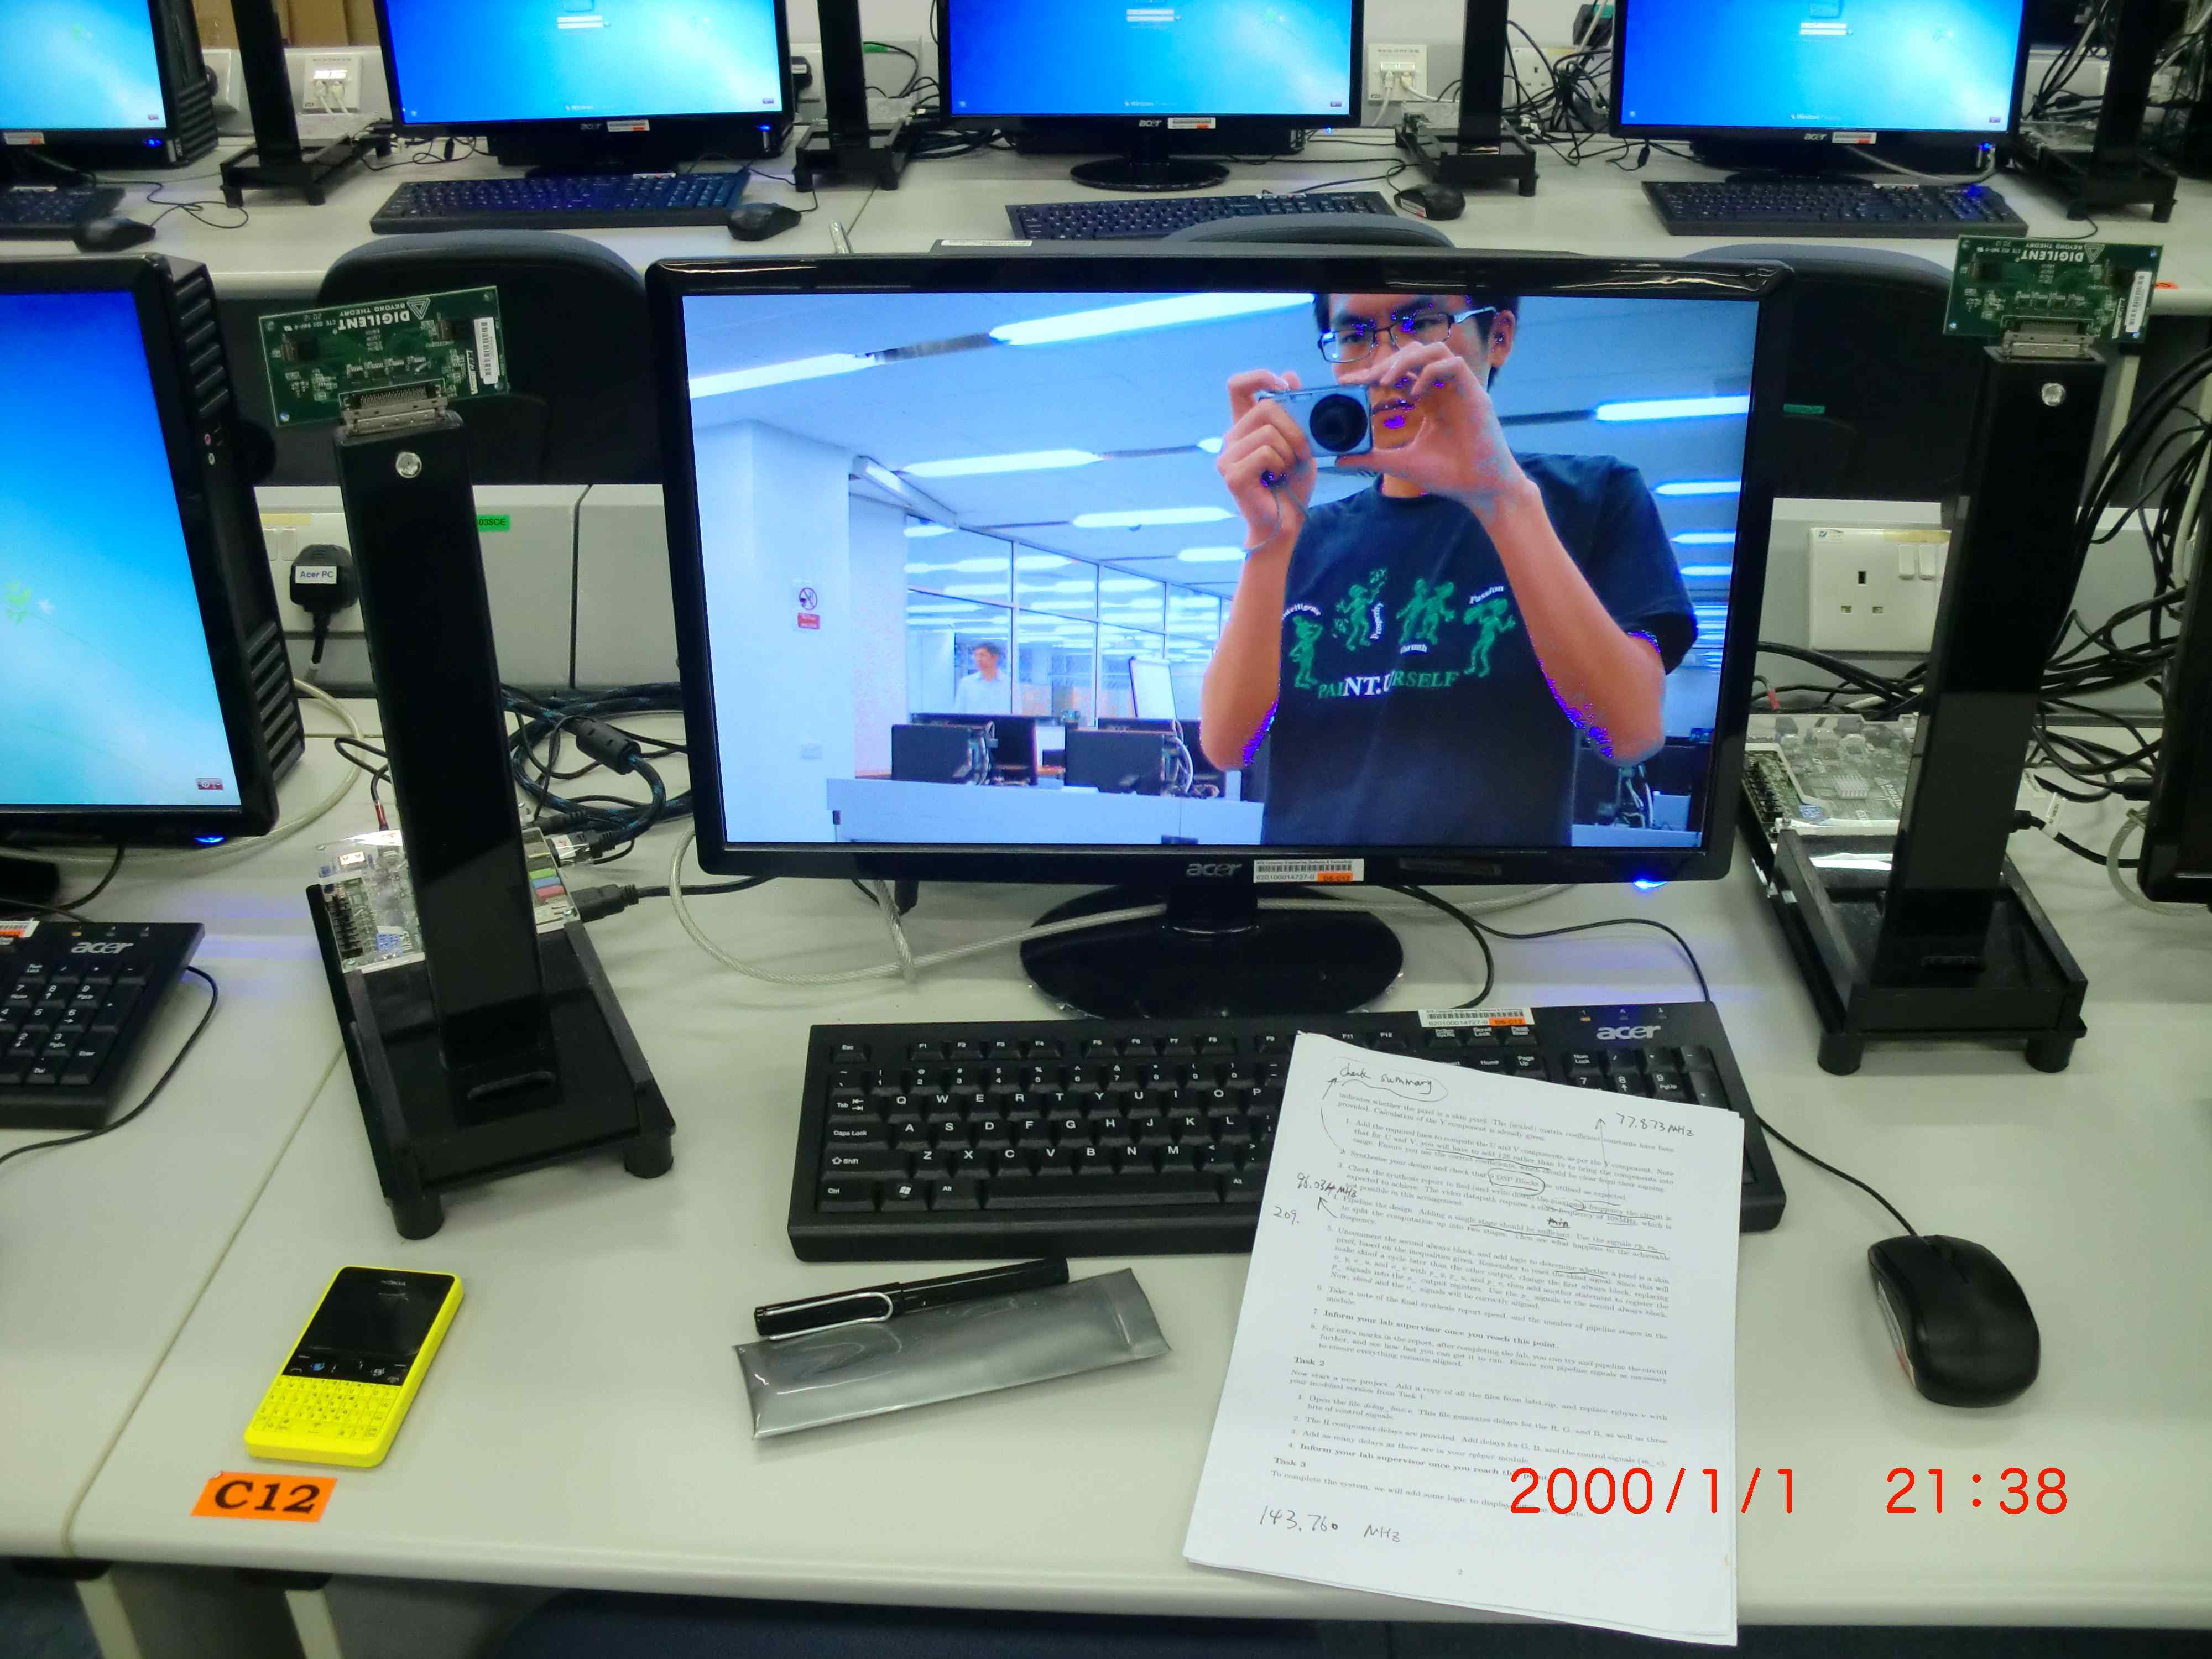
\includegraphics[width=0.5\textwidth]{a5.JPG}
\captionof{figure}{Case 16}
\end{figure}
\begin{figure}[H]
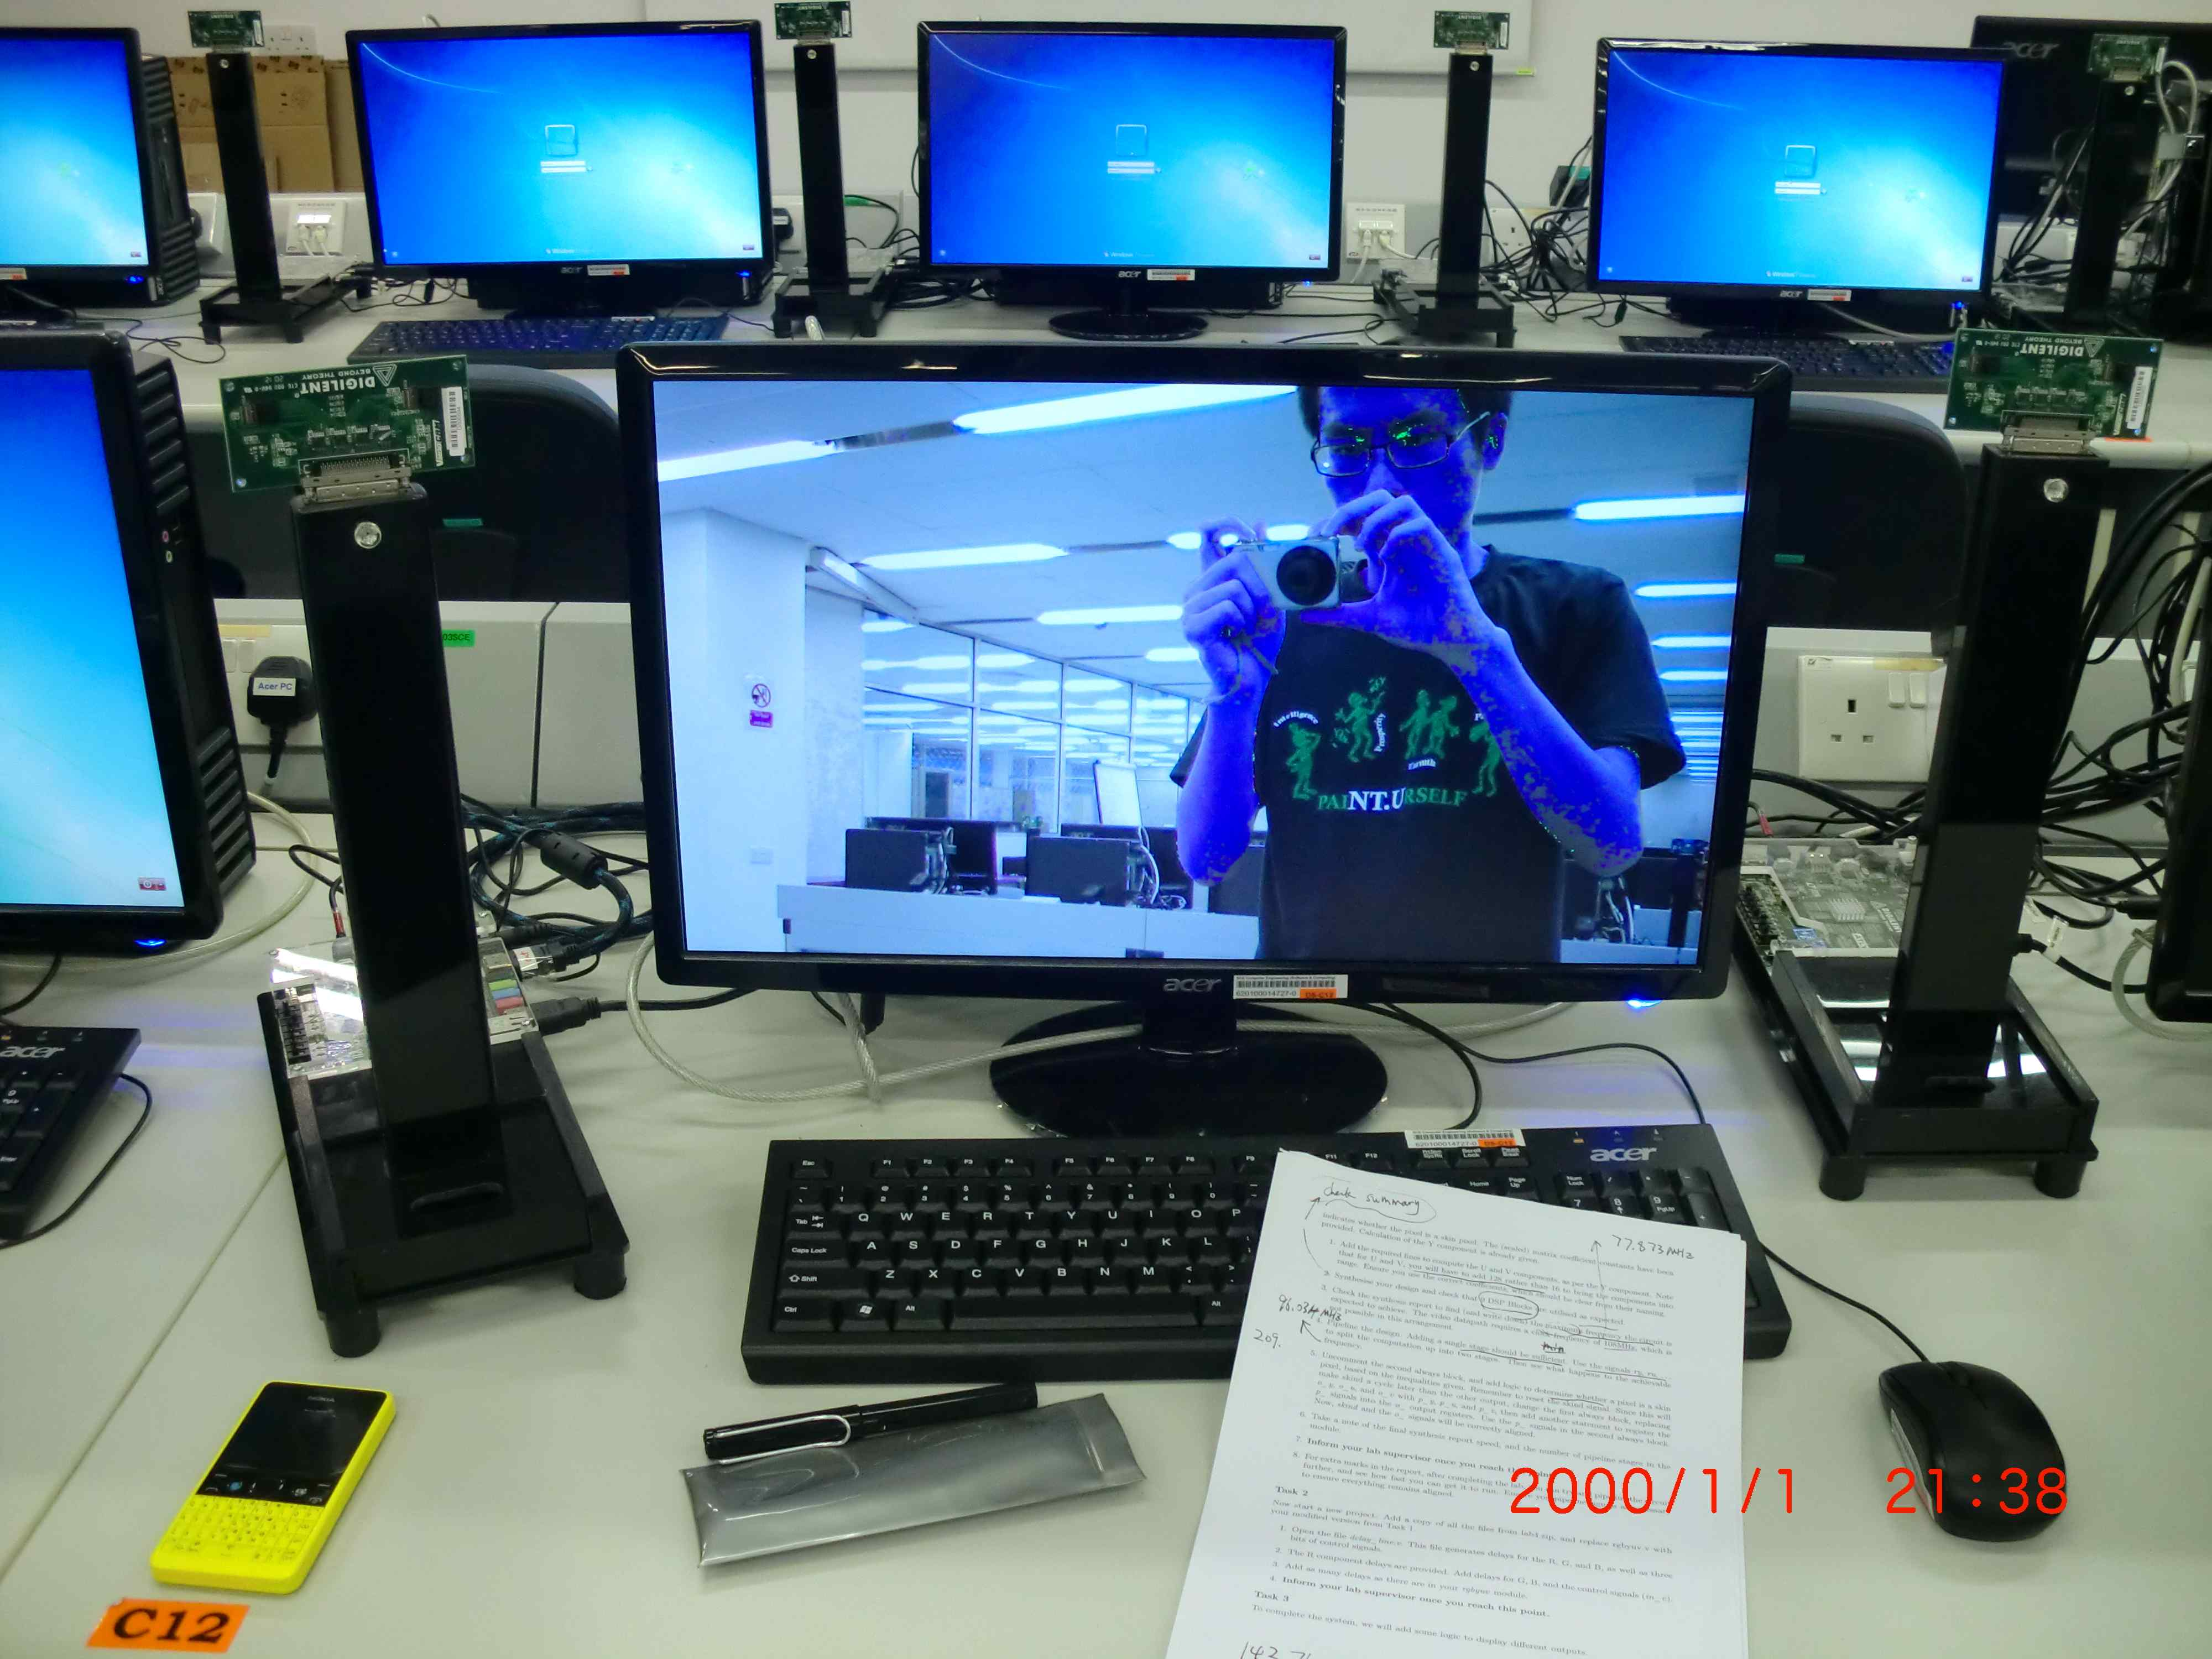
\includegraphics[width=0.5\textwidth]{a6.JPG}
\captionof{figure}{Case 32}
\end{figure}
\begin{figure}[H]
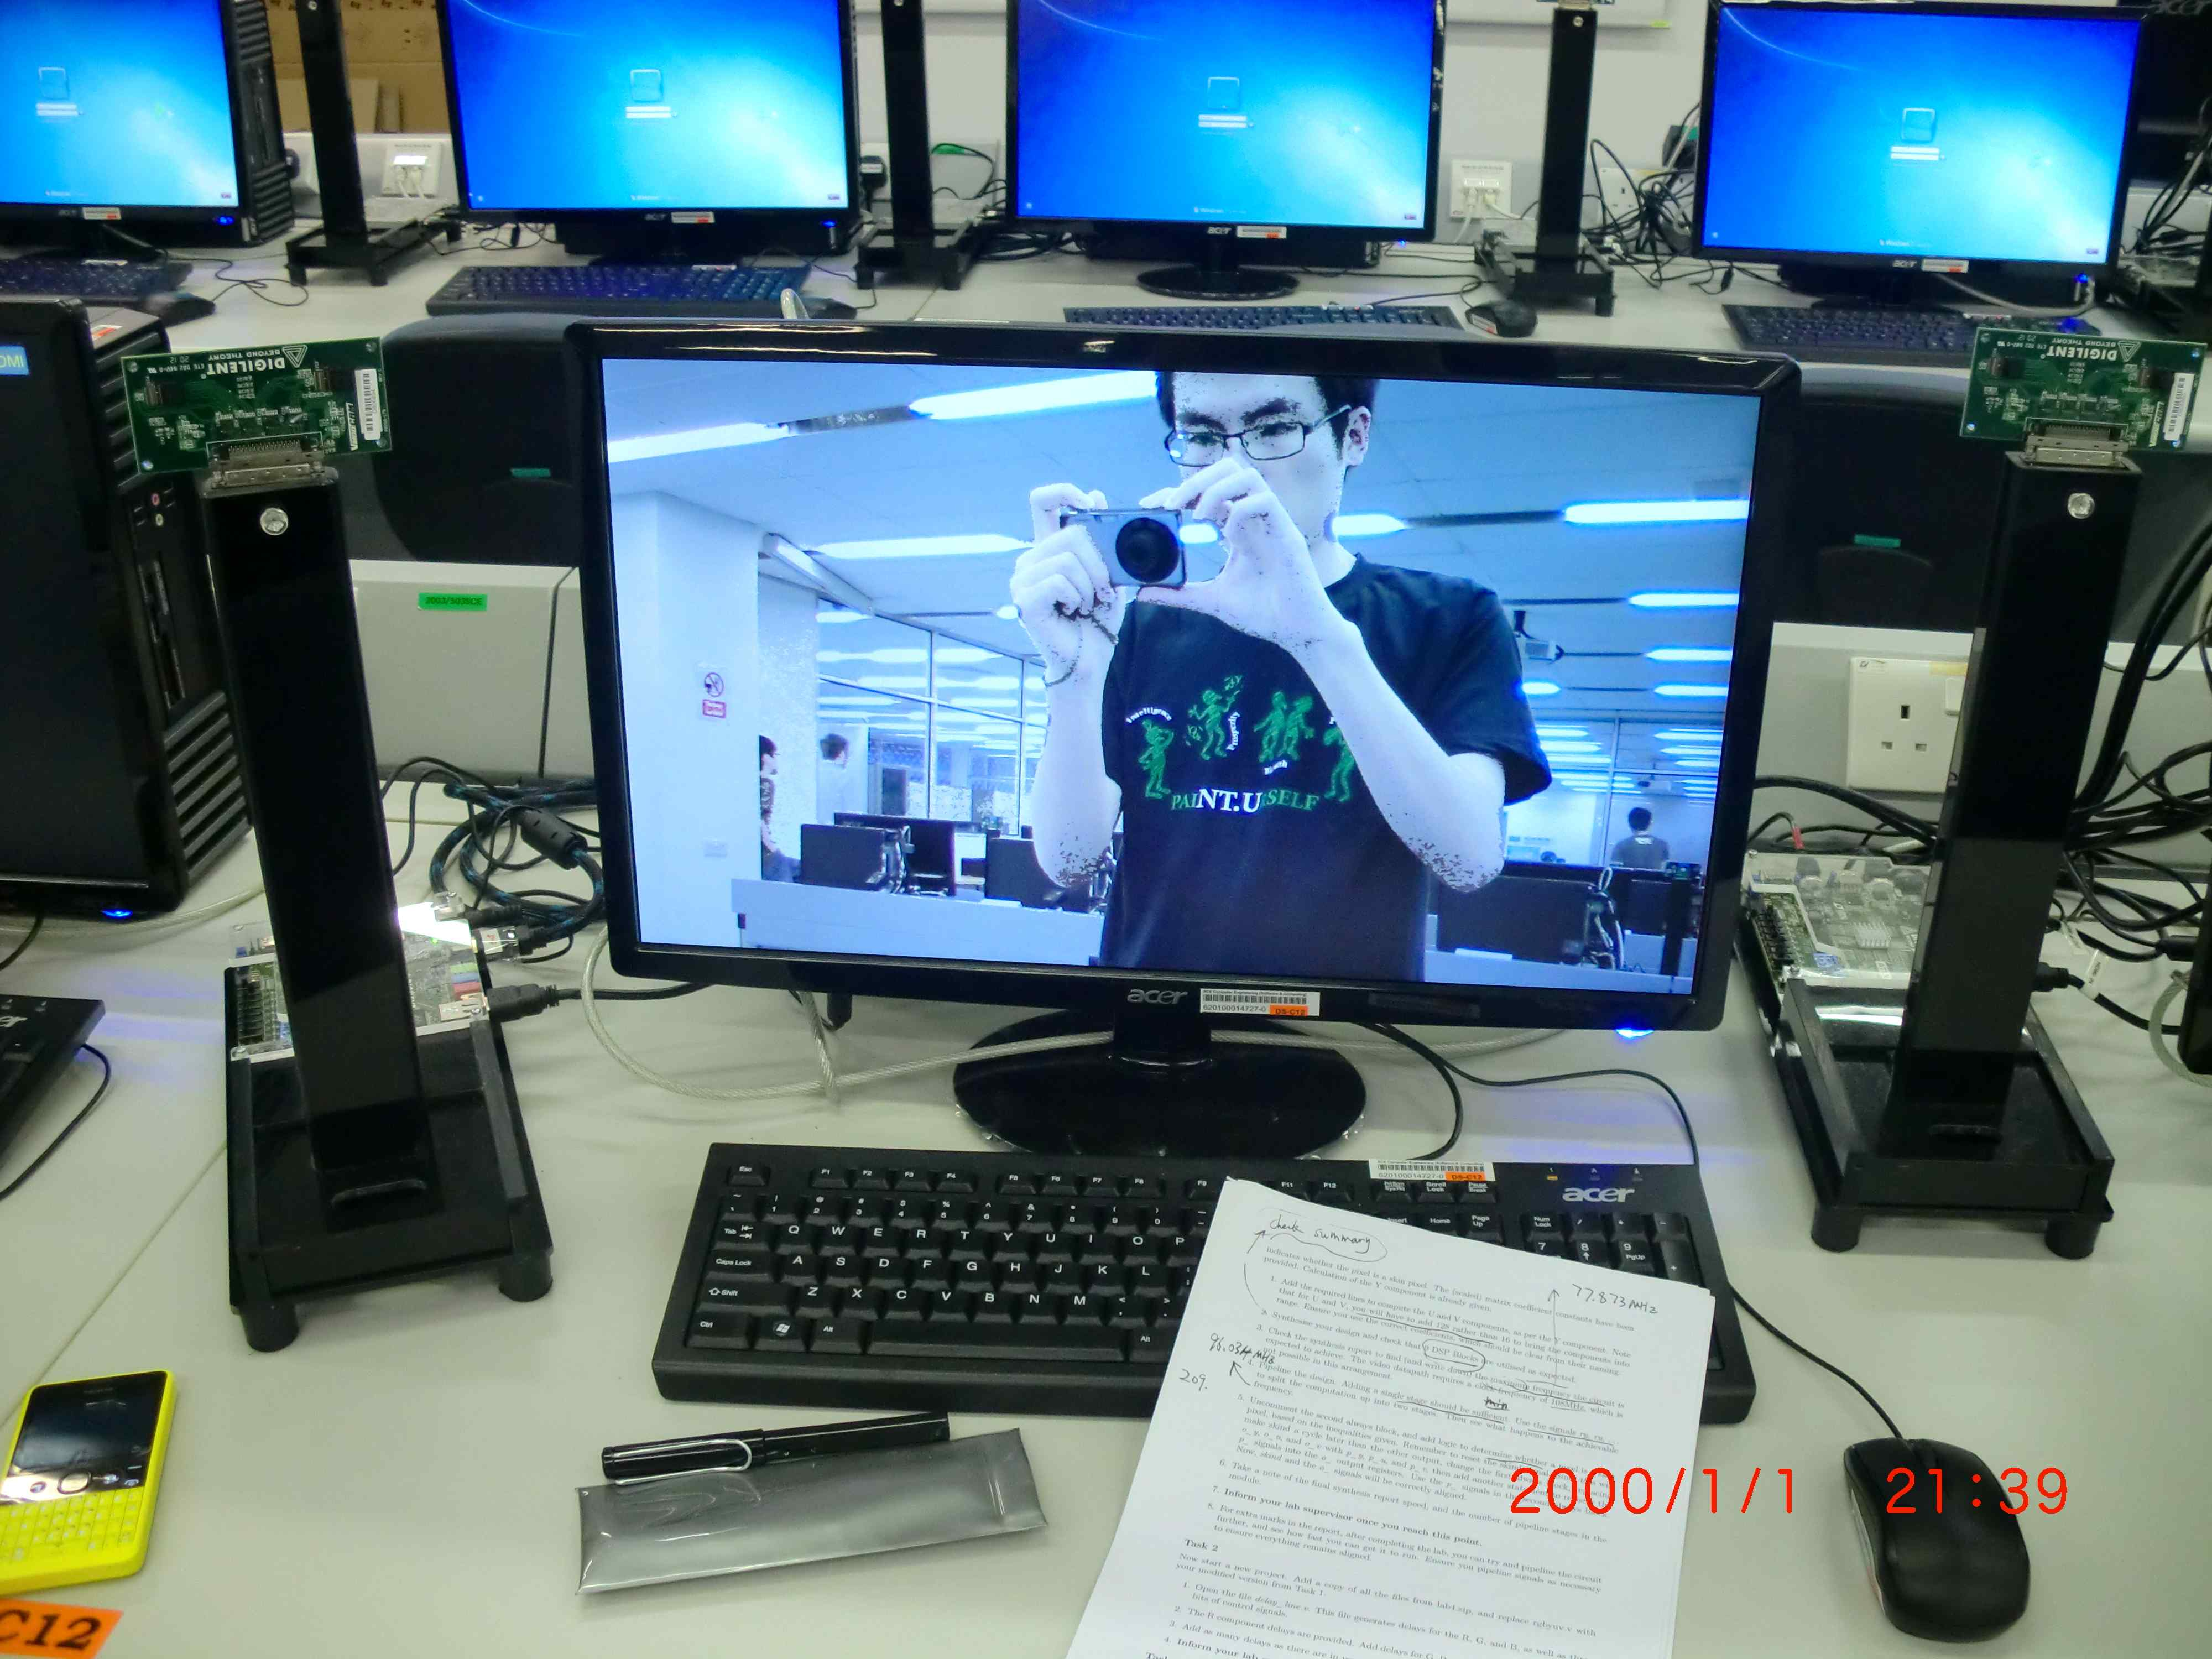
\includegraphics[width=0.5\textwidth]{a7.JPG}
\captionof{figure}{Case 64}
\end{figure}
\begin{figure}[H]
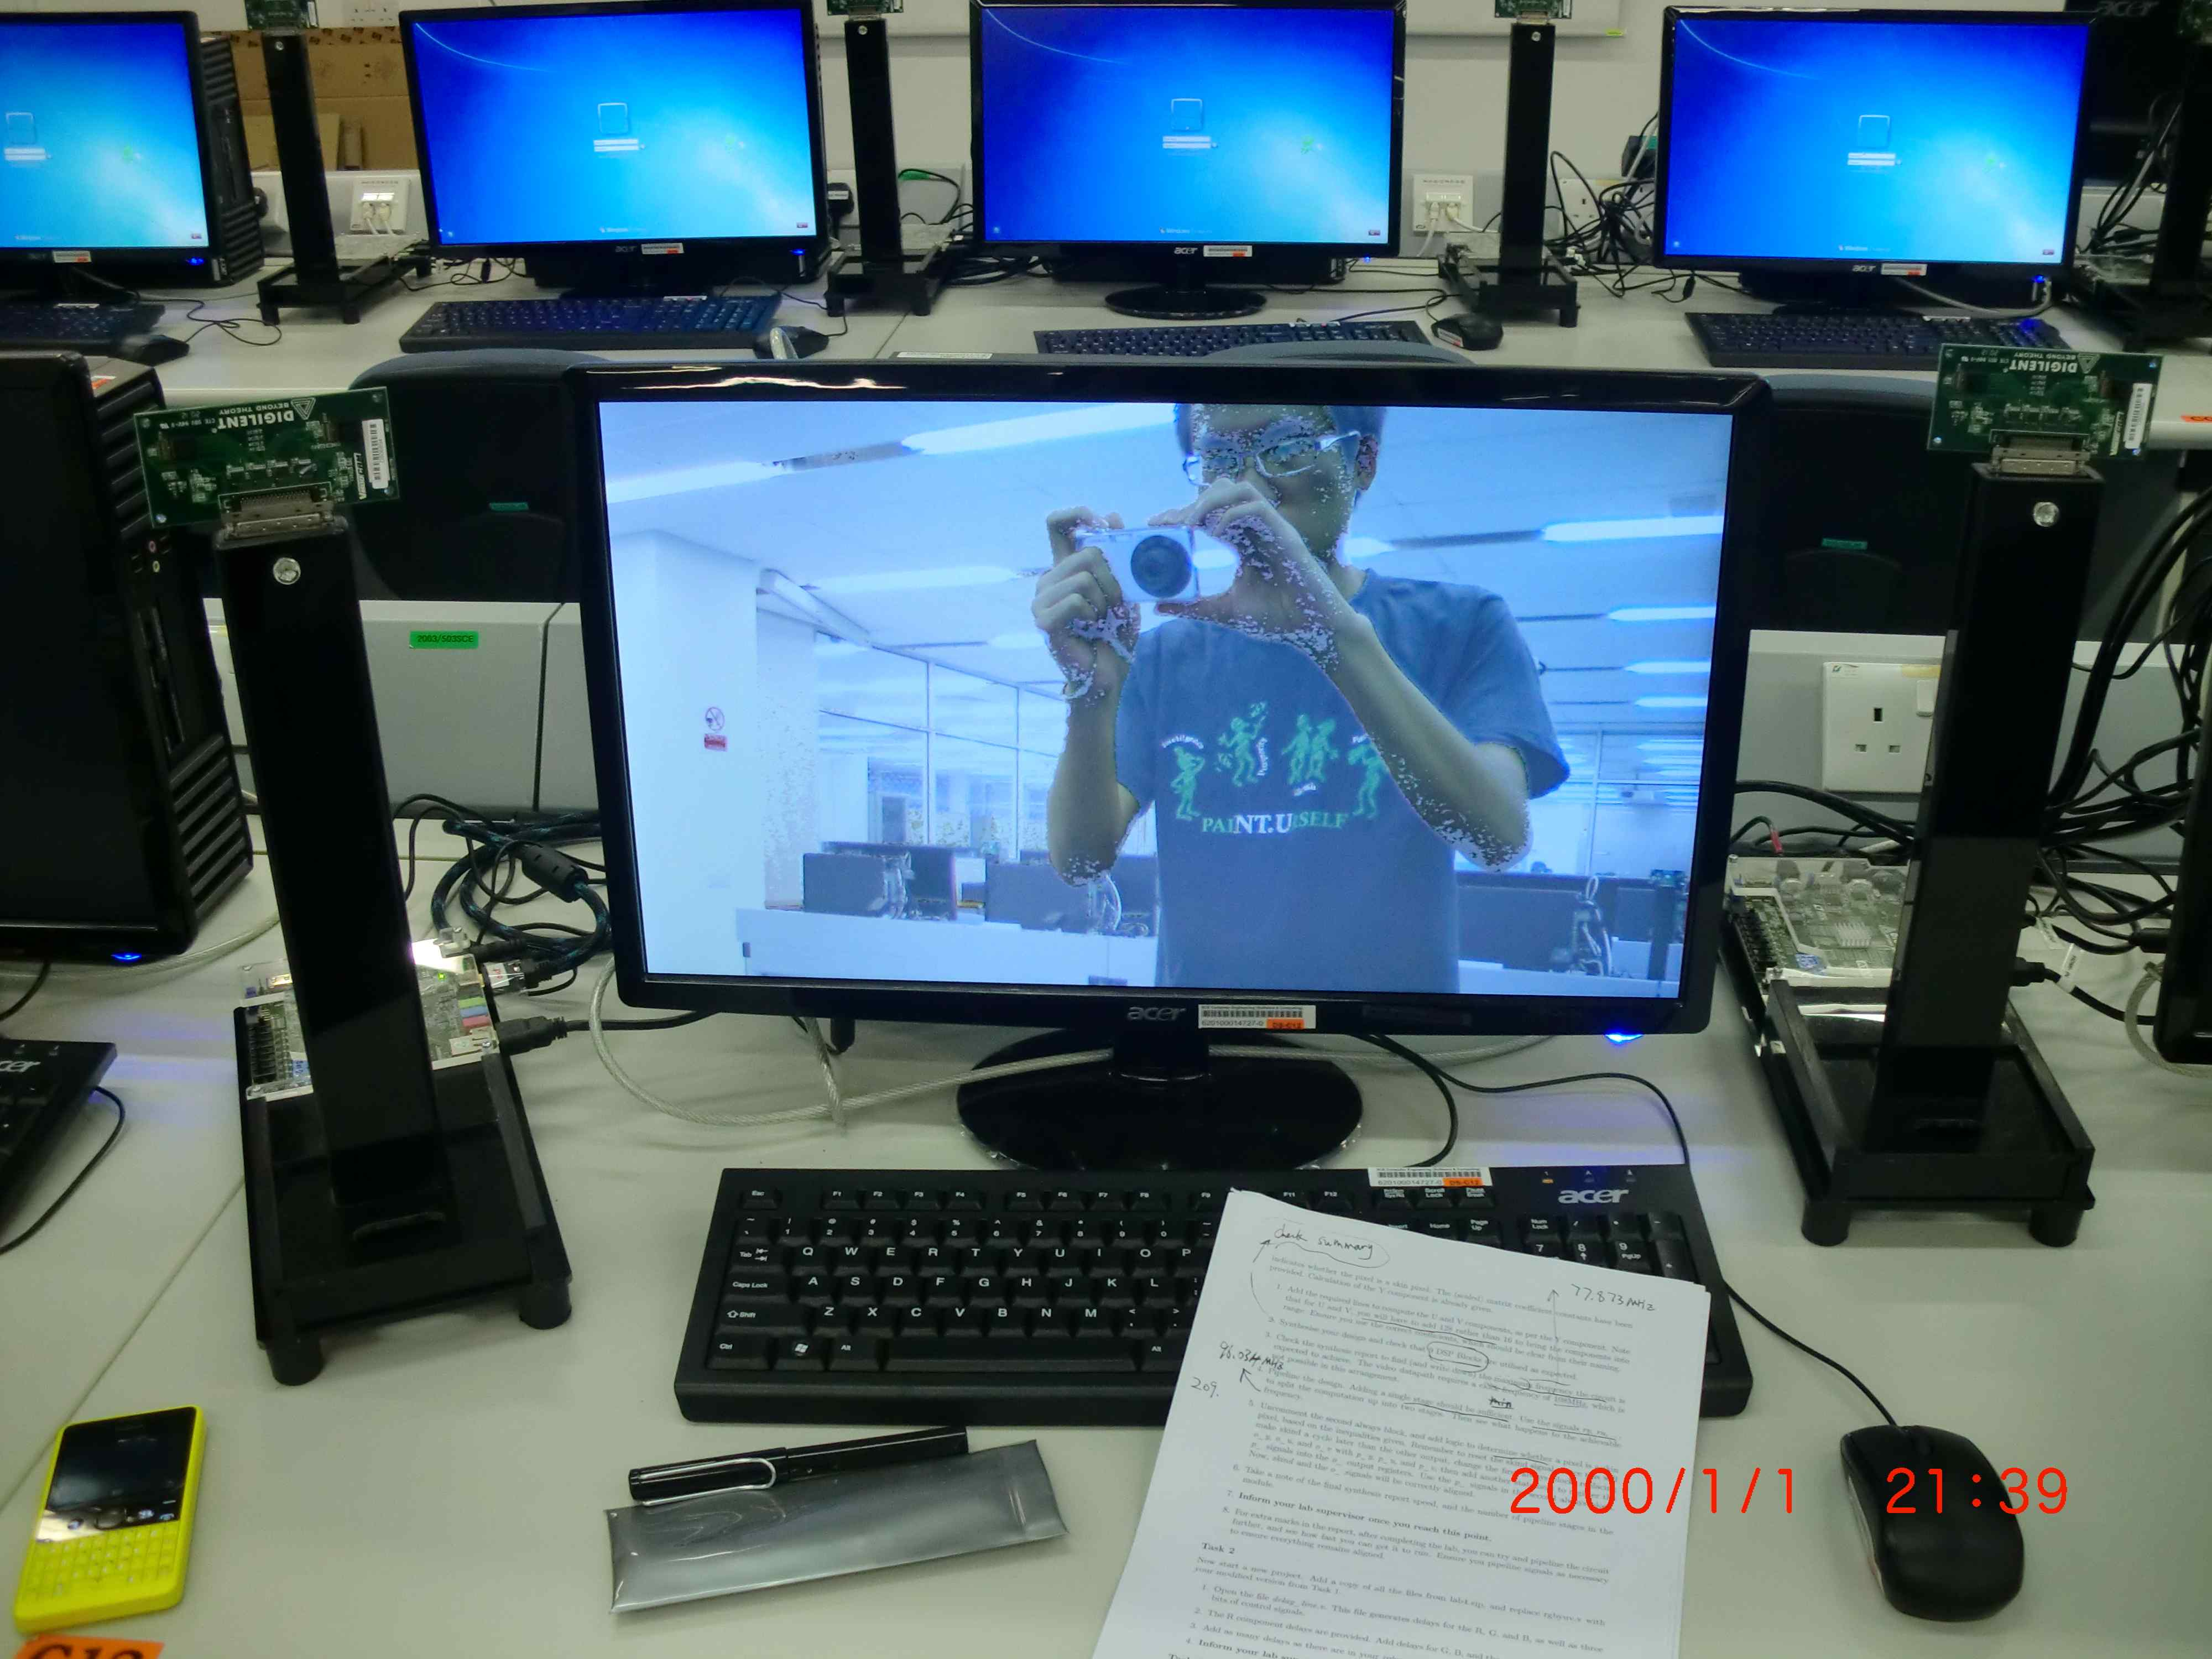
\includegraphics[width=0.5\textwidth]{a8.JPG}
\captionof{figure}{Case 128}
\end{figure}
\begin{figure}[H]
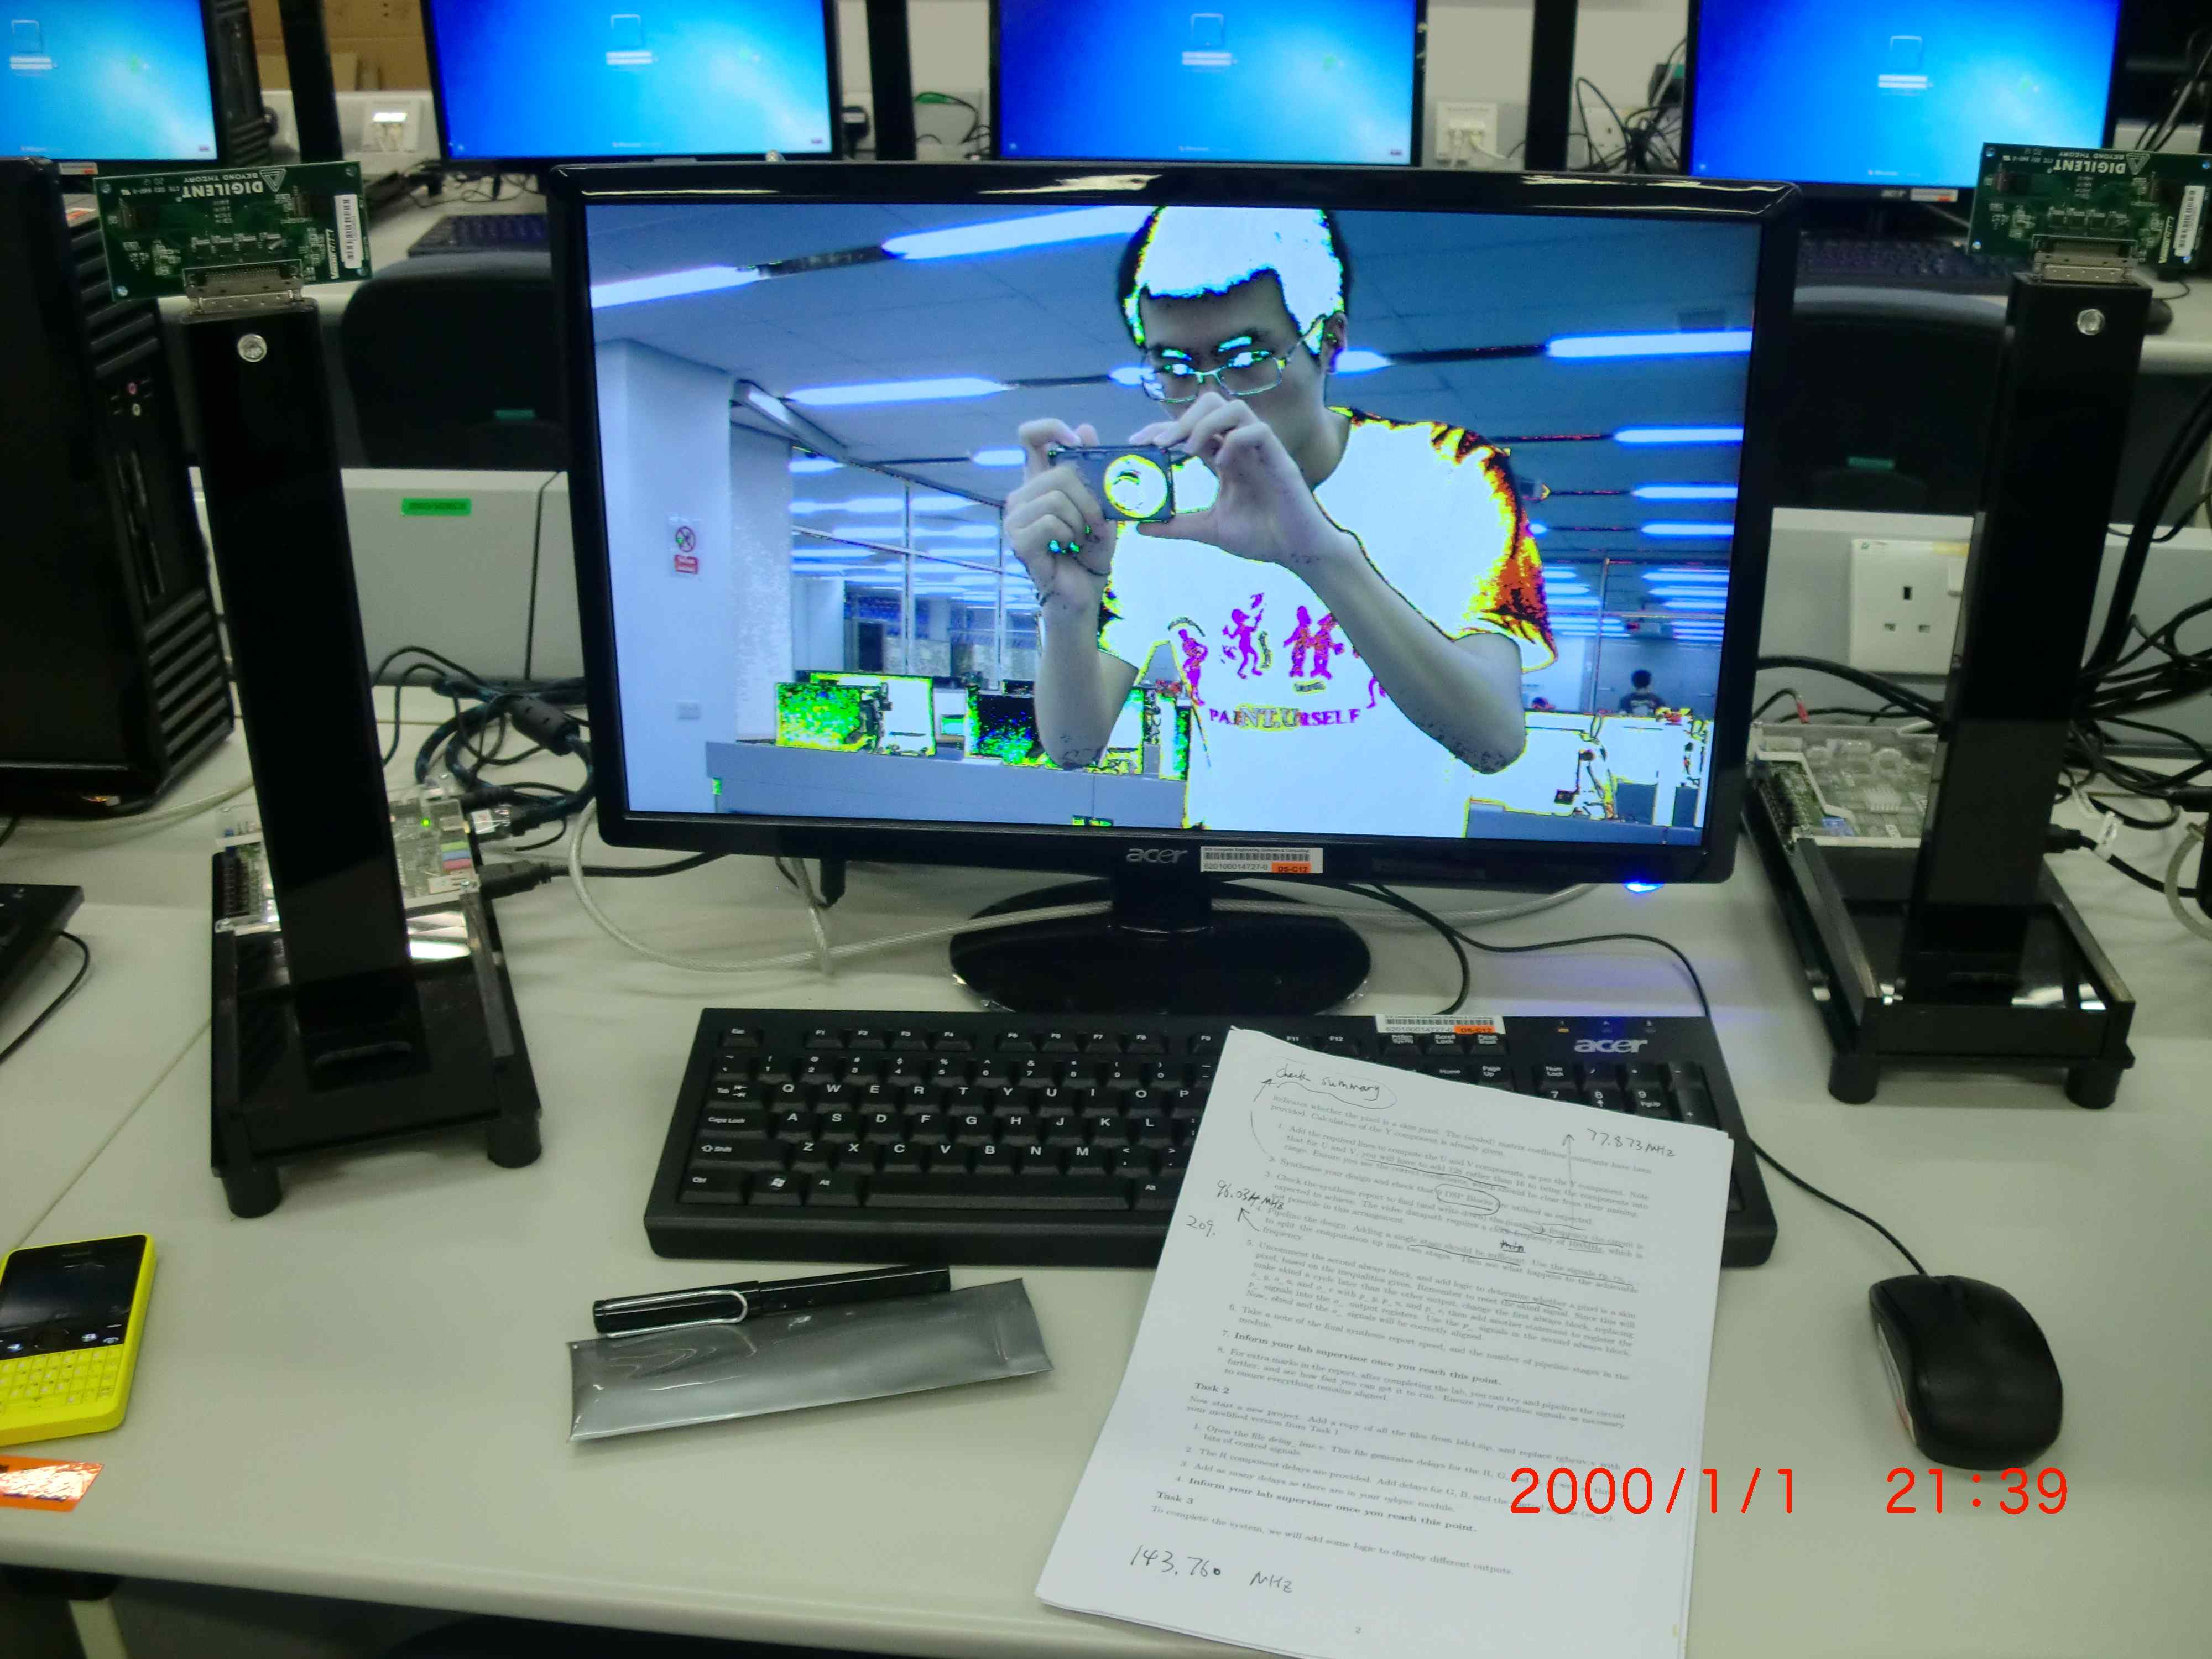
\includegraphics[width=0.5\textwidth]{a9.JPG}
\captionof{figure}{Case 255}
\end{figure}
\end{multicols}
\end{document}
